% Options for packages loaded elsewhere
\PassOptionsToPackage{unicode}{hyperref}
\PassOptionsToPackage{hyphens}{url}
\documentclass[
  12pt,
  oneside]{book}
\usepackage{xcolor}
\usepackage[left=4cm, right=3cm, top=2.5cm, bottom=2.5cm]{geometry}
\usepackage{amsmath,amssymb}
\setcounter{secnumdepth}{5}
\usepackage{iftex}
\ifPDFTeX
  \usepackage[T1]{fontenc}
  \usepackage[utf8]{inputenc}
  \usepackage{textcomp} % provide euro and other symbols
\else % if luatex or xetex
  \usepackage{unicode-math} % this also loads fontspec
  \defaultfontfeatures{Scale=MatchLowercase}
  \defaultfontfeatures[\rmfamily]{Ligatures=TeX,Scale=1}
\fi
\usepackage{lmodern}
\ifPDFTeX\else
  % xetex/luatex font selection
\fi
% Use upquote if available, for straight quotes in verbatim environments
\IfFileExists{upquote.sty}{\usepackage{upquote}}{}
\IfFileExists{microtype.sty}{% use microtype if available
  \usepackage[]{microtype}
  \UseMicrotypeSet[protrusion]{basicmath} % disable protrusion for tt fonts
}{}
\usepackage{setspace}
\makeatletter
\@ifundefined{KOMAClassName}{% if non-KOMA class
  \IfFileExists{parskip.sty}{%
    \usepackage{parskip}
  }{% else
    \setlength{\parindent}{0pt}
    \setlength{\parskip}{6pt plus 2pt minus 1pt}}
}{% if KOMA class
  \KOMAoptions{parskip=half}}
\makeatother
\usepackage{longtable,booktabs,array}
\newcounter{none} % for unnumbered tables
\usepackage{calc} % for calculating minipage widths
% Correct order of tables after \paragraph or \subparagraph
\usepackage{etoolbox}
\makeatletter
\patchcmd\longtable{\par}{\if@noskipsec\mbox{}\fi\par}{}{}
\makeatother
% Allow footnotes in longtable head/foot
\IfFileExists{footnotehyper.sty}{\usepackage{footnotehyper}}{\usepackage{footnote}}
\makesavenoteenv{longtable}
\usepackage{graphicx}
\makeatletter
\newsavebox\pandoc@box
\newcommand*\pandocbounded[1]{% scales image to fit in text height/width
  \sbox\pandoc@box{#1}%
  \Gscale@div\@tempa{\textheight}{\dimexpr\ht\pandoc@box+\dp\pandoc@box\relax}%
  \Gscale@div\@tempb{\linewidth}{\wd\pandoc@box}%
  \ifdim\@tempb\p@<\@tempa\p@\let\@tempa\@tempb\fi% select the smaller of both
  \ifdim\@tempa\p@<\p@\scalebox{\@tempa}{\usebox\pandoc@box}%
  \else\usebox{\pandoc@box}%
  \fi%
}
% Set default figure placement to htbp
\def\fps@figure{htbp}
\makeatother
% definitions for citeproc citations
\NewDocumentCommand\citeproctext{}{}
\NewDocumentCommand\citeproc{mm}{%
  \begingroup\def\citeproctext{#2}\cite{#1}\endgroup}
\makeatletter
 % allow citations to break across lines
 \let\@cite@ofmt\@firstofone
 % avoid brackets around text for \cite:
 \def\@biblabel#1{}
 \def\@cite#1#2{{#1\if@tempswa , #2\fi}}
\makeatother
\newlength{\cslhangindent}
\setlength{\cslhangindent}{1.5em}
\newlength{\csllabelwidth}
\setlength{\csllabelwidth}{3em}
\newenvironment{CSLReferences}[2] % #1 hanging-indent, #2 entry-spacing
 {\begin{list}{}{%
  \setlength{\itemindent}{0pt}
  \setlength{\leftmargin}{0pt}
  \setlength{\parsep}{0pt}
  % turn on hanging indent if param 1 is 1
  \ifodd #1
   \setlength{\leftmargin}{\cslhangindent}
   \setlength{\itemindent}{-1\cslhangindent}
  \fi
  % set entry spacing
  \setlength{\itemsep}{#2\baselineskip}}}
 {\end{list}}
\usepackage{calc}
\newcommand{\CSLBlock}[1]{\hfill\break\parbox[t]{\linewidth}{\strut\ignorespaces#1\strut}}
\newcommand{\CSLLeftMargin}[1]{\parbox[t]{\csllabelwidth}{\strut#1\strut}}
\newcommand{\CSLRightInline}[1]{\parbox[t]{\linewidth - \csllabelwidth}{\strut#1\strut}}
\newcommand{\CSLIndent}[1]{\hspace{\cslhangindent}#1}
\setlength{\emergencystretch}{3em} % prevent overfull lines
\providecommand{\tightlist}{%
  \setlength{\itemsep}{0pt}\setlength{\parskip}{0pt}}
\usepackage{fontspec}
\setmainfont{Times New Roman}[
  Ligatures = TeX
]
\setsansfont{Helvetica}[
  Scale = MatchLowercase
]
\setmonofont{Menlo}[
  Scale = MatchLowercase
]

\usepackage{titlesec}
\titleformat{\chapter}[hang]
  {\normalfont\huge\bfseries}
  {\chaptertitlename~\thechapter}
  {1em}
  {}
\titlespacing*{\chapter}{0pt}{50pt}{40pt}

\usepackage[none]{hyphenat}
\pagestyle{plain}
\raggedbottom
\usepackage[nottoc,notlot,notlof]{tocbibind}
\usepackage{pdfpages}
\usepackage[width=\textwidth]{caption}

\usepackage{fancyhdr}
\pagestyle{fancy}
\fancyhf{}
\setlength{\headheight}{15pt}%
\fancyhead[RO,RE]{\nouppercase{\leftmark}}
\fancyfoot[CO, CE] {\thepage}
\renewcommand{\headrulewidth}{0pt}
\renewcommand{\footrulewidth}{0pt}

% Handbook: Arabic numerals from the cover through the last appendix, with
% no roman front matter and no restart at Chapter 1.
\AtBeginDocument{\pagenumbering{arabic}}
\makeatletter
\renewenvironment{titlepage}{%
  \if@twocolumn
    \@restonecoltrue\onecolumn
  \else
    \@restonecolfalse\newpage
  \fi
  \thispagestyle{plain}%
  \setcounter{page}{\@ne}%
}{%
  \if@restonecol\twocolumn \else \newpage \fi
}
\makeatother
\usepackage{bookmark}
\IfFileExists{xurl.sty}{\usepackage{xurl}}{} % add URL line breaks if available
\urlstyle{same}
% fallback for those not using the hyperref driver hyperxmp:
\makeatletter
\@ifundefined{xmpquote}{\newcommand{\xmpquote}[1]{#1}}{}
\makeatother
\hypersetup{
  pdftitle={A Modality-Aware Spatio-Temporal Fusion Framework for Brent Crude Oil Forecasting Using Financial Time Series{,} Satellite Imagery and Maritime Networks},
  hidelinks,
  pdfcreator={LaTeX via pandoc}}

\title{A Modality-Aware Spatio-Temporal Fusion Framework for Brent Crude Oil Forecasting Using Financial Time Series, Satellite Imagery and Maritime Networks}
\author{XINRUI QI\\
\strut \\
CASA0004, MSc Dissertation\\
\strut \\
Supervisor: Beatrice Taylor\\
\strut \\
Code repository: \url{https://github.com/XINRUIQI/CASA0004-Dissertation}\\
\strut \\
This dissertation is submitted in part requirement for the\\
MSc in the Centre for Advanced Spatial Analysis,\\
Bartlett Faculty of the Built Environment, UCL\\
\strut \\
Word count: 10800??}
\date{2026-08-17}

\begin{document}
\maketitle

\setstretch{1.5}
\chapter*{Abstract}\label{abstract}

Brent crude is one of the principal benchmarks for internationally traded oil and a key reference price in the global energy market. Its short-term movements affect energy costs, inflation, trade balances and fiscal revenues, and therefore influence decisions made by firms and governments. Using weekly data from 2019 to 2025, this study examines whether satellite remote-sensing and shipping data provide incremental value beyond financial time series for one-week-ahead Brent price forecasting. It also compares flat feature fusion with modality-specific encoding followed by fusion. Flat models combine all selected inputs in a single feature table, whereas deep models encode each data source separately before fusing the resulting representations. For both model families, the study compares a financial-time-series-only specification with alternatives that add remote sensing, shipping or both.

The models are evaluated against a no-change benchmark that sets next week's price equal to this week's price. The results show that no flat model outperforms this benchmark, although shipping data provide limited evidence of incremental predictive information. Deep models combining financial time series and shipping data achieve a small improvement over the benchmark. Remote-sensing data provide no clear additional benefit. The advantage of deep models over flat models is most evident when shipping data are included. This study further uses modality gates to show which data sources the best-performing deep model relies on most. Overall, predictive value depends more on how multimodal data are used---especially how modalities are encoded and fused---than on simply adding more data.

\chapter*{Declaration}\label{declaration}

I hereby declare that this dissertation is all my own original work and that all sources have been acknowledged. It is xxx words in length.

\chapter*{Acknowledgements}\label{acknowledgements}

I would like to thank my supervisor and those who supported this dissertation.

\setcounter{tocdepth}{3}
\tableofcontents
\listoffigures
\listoftables

\chapter*{Abbreviations}\label{abbreviations}

{\def\LTcaptype{none} % do not increment counter
\begin{longtable}[]{@{}ll@{}}
\toprule\noalign{}
Term & Definition \\
\midrule\noalign{}
\endhead
\bottomrule\noalign{}
\endlastfoot
AIS & Automatic Identification System \\
AOI & Area of interest \\
EIA & U.S. Energy Information Administration \\
GFW & Global Fishing Watch \\
RMSE & Root mean squared error \\
SHAP & SHapley Additive exPlanations \\
WTI & West Texas Intermediate \\
\end{longtable}
}

\chapter{Introduction}\label{intro}

\section{Importance and background}\label{intro-background}

Crude oil occupies a central place in the global economy and energy system. Oil-price movements affect inflation, trade balances, fiscal revenues in producer countries and the operating costs of energy-intensive industries. These effects spread through financial markets, economic activity and supply chains. They therefore shape the risk management, hedging, budgeting and planning decisions of governments, firms and investors.

Crude oil is not a homogeneous commodity: individual grades differ in density, sulphur content, production location and transport accessibility, and their prices are commonly expressed relative to a small number of benchmarks. Among the most widely used benchmarks are Brent, West Texas Intermediate (WTI) and Dubai/Oman (\citeproc{ref-eia2014}{U.S. Energy Information Administration, 2014}). Brent is a benchmark complex rooted in light, low-sulphur, waterborne crude oils from the North Sea. It is widely used as a reference for internationally traded crude. WTI is a US crude benchmark, with pricing centred on Cushing, Oklahoma, while Dubai/Oman is commonly used to price Middle Eastern crude exported to Asian markets (\citeproc{ref-wittner2020}{Wittner, 2020}). Although Brent and WTI respond to many of the same global market conditions, differences in regional supply, inventory levels and transport constraints can cause their prices to diverge. This dissertation forecasts Brent because its role as an international waterborne benchmark aligns more closely with the ports, shipping routes and maritime chokepoints represented in the spatial data. WTI is nevertheless retained as a financial predictor and as a component of the Brent--WTI spread. No fixed volatility ranking between Brent and WTI is assumed. Whether shipping activity contains incremental predictive information for Brent is tested empirically in this dissertation.

Recent years have shown the costs of unexpected oil-price movements. The COVID-19 period brought an abrupt collapse in demand and an uneven recovery. The 2022 energy crisis then produced major supply and price shocks, followed by only partial normalisation amid continued geopolitical and macroeconomic uncertainty. More recent geopolitical disruptions have further shown how quickly oil prices and seaborne trade can respond when key maritime chokepoints are disrupted or bypassed. Governments monitor such shocks for inflation control, fiscal planning, energy security and trade policy. A better short-term oil-price model would help them gauge risk and timing. Although they cannot replace market judgement, such forecasts could support decision-making when physical flows and prices move together.

At the weekly horizon, the no-change forecast is difficult to outperform. This simple method predicts that next week's price will be equal to this week's price. It therefore provides a demanding benchmark for spatial data and forecasting methods. A model should not be considered useful merely because it outperforms a weaker or differently specified competitor. It must also be evaluated directly against the no-change benchmark.

The three data sources considered in this dissertation provide complementary views of the oil system. Financial, macroeconomic and oil-market variables describe changes in market conditions over time. Remote sensing provides geographically explicit indicators of industrial activity at eleven oil-related sites through spectral indices, night-time lights and image representations. AIS and PortWatch data provide geographically explicit observations of vessel activity across ports and six major maritime chokepoints. The shipping data also represent network relationships between locations and provide proxies for seaborne trade flows and congestion. Although Brent is observed as a single global benchmark, the underlying processes of oil production, refining and maritime transport are geographically distributed. The spatial-data inputs are therefore organised around spatially distributed monitoring sites and connected transport nodes, linking site- and network-level observations to a common forecasting target. In this dissertation, multimodal forecasting refers to combining temporal market data, spatial Earth-observation data and spatiotemporal shipping-network data within the same forecasting task.

These data create two practical challenges. First, the signals are noisy and arrive on different schedules. They may also respond to oil prices rather than predict them, while the available weekly sample is relatively small. Second, a common approach places all heterogeneous inputs in a single feature table before modelling. This flat feature-fusion approach is convenient for conventional models such as Ridge regression and gradient-boosted trees. However, it does not explicitly preserve the temporal structure of financial time series, the site structure of remote sensing or the network structure of shipping data.

This dissertation therefore addresses two empirical questions. First, do remote-sensing and shipping data improve one-week-ahead Brent price forecasts when they are added to financial time series? Can the resulting models outperform the no-change benchmark? Second, when the underlying data remain the same, does encoding each modality separately before fusion perform better than combining all inputs in a single feature table? The next section presents the study aim and formal research questions.

\section{Aim and research questions}\label{intro-aim}

The main aim of this dissertation is to develop a reproducible comparison framework for evaluating how different data sources and model designs perform in one-week-ahead Brent price forecasting. The framework combines financial time-series data, satellite remote-sensing data and shipping data. It uses a rolling-origin design that restricts each forecast to information available at the forecast origin and compares models by forecast accuracy. Flat feature fusion places all inputs in a single feature table before modelling. Representation-level fusion encodes each modality separately and then combines the resulting representations. This framework enables consistent comparisons of the incremental value of different data sources and the effects of different fusion designs. The empirical setting uses weekly Friday-ending Brent spot prices from 2019 to 2025, spanning periods of demand, supply and maritime disruption, with remote-sensing and shipping inputs covering eleven oil-related monitoring sites and six major maritime chokepoints.

The study is organised around three research questions.

\textbf{RQ1.} Compared with models using only financial time-series data, do remote-sensing and shipping data improve one-week-ahead Brent price forecasts?

\textbf{RQ2.} When using the same underlying data, does modality-aware representation-level fusion outperform flat feature fusion?

\textbf{RQ3.} Which data sources and spatial nodes do the models rely on, and how does this reliance vary across forecast periods?

\chapter{Literature review}\label{literature}

This chapter reviews the main bodies of literature that support the study. It first examines the economic drivers and empirical benchmarks of crude-oil price forecasting, followed by the application of machine-learning methods. It then reviews how shipping activity reflects oil-market conditions and how satellite remote sensing provides oil-market information. Next, it introduces multimodal learning and fusion methods. Finally, it identifies the research gaps and positions this dissertation within the existing literature.

\section{Crude-oil price drivers and forecasting benchmarks}\label{lit-benchmarks}

Research on oil-price movements shows that similar price changes can arise from economically different sources. Kilian (\citeproc{ref-kilian2009}{2009}) distinguishes among shocks to global crude-oil production, shocks to aggregate demand for industrial commodities and demand shocks specific to the oil market. Oil prices respond differently to these shocks, and each shock has a different relationship with global economic activity and oil production. This distinction provides an economic basis for using variables related to supply, demand, market expectations and macroeconomic conditions in oil-price forecasting.

A separate literature examines whether these economic relationships produce accurate forecasts. Alquist, Kilian and Vigfusson (\citeproc{ref-alquist2013}{2013}) compare a wide range of forecasting models with the no-change forecast, which sets the future spot price equal to the current price. Many alternative models fail to outperform this simple benchmark consistently, particularly in real-time and out-of-sample evaluations. They also distinguish economic predictability from practical forecastability. A variable may have an economic relationship with future oil prices without reducing forecast errors in a finite out-of-sample period. Baumeister and Kilian (\citeproc{ref-baumeister2015}{2015}) find that combining forecasts from several econometric models can produce more stable results across periods and forecast horizons than relying on a single model. These studies establish the no-change forecast as an important benchmark and show that model performance can vary substantially across evaluation periods.

\section{Machine learning in crude-oil price forecasting}\label{lit-ml}

Machine learning has expanded the range of methods used in oil-price forecasting. These methods can process large predictor sets and capture nonlinear relationships and interactions. Costa \emph{et al.} (\citeproc{ref-costa2021}{2021}) evaluate 23 methods using 315 macroeconomic and financial variables. They find that no single method performs best at every forecast horizon. Machine-learning methods are competitive at short horizons, but econometric, market-based and combined forecasts also perform strongly in some settings. Yılmaz and Zehir (\citeproc{ref-yilmaz2026}{2026}) compare econometric and tree-based models for Brent returns using macro-financial and geopolitical variables. Light Gradient Boosting Machine (LightGBM) produces the most consistent results across their reported settings, but the broader comparison again shows that performance depends on the forecast horizon, predictor set and evaluation design.

Deep-learning studies focus more directly on learning temporal representations. Foroutan and Lahmiri (\citeproc{ref-foroutan2024}{2024}) compare a range of methods for next-day WTI and Brent spot-price forecasting and report strong performance from temporal convolutional networks and LightGBM. Simsek \emph{et al.} (\citeproc{ref-simsek2024}{2024}) combine Long Short-Term Memory (LSTM) feature extraction with XGBoost for WTI price prediction. Graph-based methods have also been introduced. Zhao, Xue and Cheng (\citeproc{ref-zhao2023}{2023}), for example, model time-varying relationships among economic and financial variables and use a spatial--temporal graph neural network to forecast WTI futures. Their graph represents statistical relationships among predictors rather than a physical transportation network.

Overall, machine learning provides greater flexibility for modelling high-dimensional data, nonlinearities and temporal interactions. However, the literature does not establish that one class of models consistently dominates conventional econometric or market-based approaches. Reported performance depends strongly on the target, horizon, sample, information set and benchmark. These findings support the use of a common rolling out-of-sample design and a no-change benchmark when comparing different data sources and model architectures.

\section{Shipping activity as an oil-market signal}\label{lit-shipping}

A large share of international crude-oil trade is transported by sea. Shipping activity can therefore provide information about physical oil flows, regional supply conditions, congestion and disruptions at ports or major chokepoints. Automatic Identification System (AIS) data record vessel identities, positions and movements. Although they do not directly record cargo quantities, processed AIS observations can be used to estimate tanker movements and maritime trade.

Adland, Jia and Strandenes (\citeproc{ref-adland2017}{2017}) compare AIS-based estimates of seaborne crude-oil exports with customs statistics and find that aggregate estimates are broadly consistent with official data. Yan \emph{et al.} (\citeproc{ref-yan2020}{2020}) combine tanker trajectories with vessel characteristics and draught information to estimate voyage-level oil flows. Their estimates for major oil-importing and oil-exporting countries are strongly correlated with Joint Organisations Data Initiative statistics. These studies provide evidence that vessel movements can serve as proxies for the physical transportation of crude oil.

AIS-based indicators can also improve the timeliness of trade measurement. Arslanalp, Marini and Tumbarello (\citeproc{ref-arslanalp2019}{2019}) construct high-frequency trade indicators from vessel movements and port calls. IMF PortWatch extends this approach by combining information on vessel activity, ports, chokepoints, ship characteristics and estimated carrying capacity to produce daily indicators of maritime trade (\citeproc{ref-arslanalp2026}{Arslanalp \emph{et al.}, 2026}). Compared with conventional trade statistics, these data can describe changes in maritime activity with shorter reporting delays.

However, the relationship between shipping activity and future oil prices is not necessarily one-directional. Mi \emph{et al.} (\citeproc{ref-mi2022}{2022}) identify relationships between oil-price changes and tanker port-call frequency, docking time, gross tonnage and the number of tankers at ports in major crude-exporting countries. Mi \emph{et al.} (\citeproc{ref-mi2023}{2023}) also find nonlinear and regionally heterogeneous relationships between oil prices and tanker port calls. In both studies, shipping activity responds to oil prices. Their results therefore show that contemporaneous associations do not establish that vessel activity leads future price movements.

AIS-based measures are also indirect and incomplete. Cargo type and quantity must often be inferred from vessel characteristics, routes or draught, and some vessel activity is not observed in public tracking systems. Paolo \emph{et al.} (\citeproc{ref-paolo2024}{2024}) show that a meaningful share of transport- and energy-vessel activity is absent from public vessel-position data. These limitations do not make AIS data unusable, but they mean that shipping variables should be treated as noisy proxies for physical trade rather than direct measurements of oil supply.

The existing literature establishes that shipping data can measure changes in maritime trade and crude-oil transportation. However, direct evidence that these data improve short-term Brent price forecasts remains limited.

\section{Maritime networks and graph-based modelling}\label{lit-networks}

Maritime-network studies provide a way to preserve relationships among locations. Aggregate indicators summarise port calls, vessel counts or chokepoint traffic, whereas network models represent ports or regions as nodes and vessel movements as links. This representation retains connections between locations and allows activity at one part of the network to be modelled in relation to activity elsewhere.

Ouyang \emph{et al.} (\citeproc{ref-ouyang2022}{2022}) construct a crude-oil transportation network and use an LSTM--GCN model to forecast weekly traffic at network nodes. Liang \emph{et al.} (\citeproc{ref-liang2022}{2022}) use a spatiotemporal multigraph convolutional network for vessel-traffic forecasting, while Zhao \emph{et al.} (\citeproc{ref-zhao2022}{2022}) use a dynamic graph neural network to predict regional vessel inflows, outflows and traffic volumes. These studies show that maritime activity is relational and changes over time. Preserving this structure may therefore provide information that is lost when shipping activity is reduced to a small set of aggregate indicators.

The literature shows that network representations can capture relationships between ports and routes. However, these methods have mainly been used to forecast shipping activity itself. There is limited direct evidence on whether graph-based representations of maritime networks improve oil-price forecasts.

\section{Remote sensing as an oil-market signal}\label{lit-remote}

Remote sensing provides repeated observations of oil-related infrastructure, industrial activity and maritime locations. Satellite observations may therefore contain information about oil demand, storage, port activity and trade. However, their economic meaning depends on the physical signal being measured and the mechanism connecting that signal to the oil market.

Several studies connect satellite observations with oil-market conditions. Hao and Wang (\citeproc{ref-hao2023}{2023}) use cloud-cover observations above floating-roof oil tanks in major US storage areas. Because the roofs rise and fall with the volume of oil stored, their shadows in clear-sky satellite imagery can be used to estimate inventories before official EIA releases. Cloud cover obscures the tanks and therefore reduces the satellite-based inventory information available to market participants. The authors argue that the resulting information uncertainty may encourage firms to hold larger precautionary inventories. Consistent with this proposed channel, they find that greater cloud cover is followed by higher inventories and lower WTI returns in the following week. They interpret this as an information effect rather than a direct weather effect on oil supply or demand. Bricongne \emph{et al.} (\citeproc{ref-bricongne2026}{2026}) use satellite observations of tropospheric NO₂, a short-lived pollutant emitted primarily by fossil-fuel combustion, to nowcast national oil demand. They find that daily NO₂ data improve nowcasting accuracy relative to models using conventional predictors, showing that satellite observations can provide timely information about changes in oil consumption.

Other studies use satellite imagery to measure oil-related infrastructure and trade. Wang \emph{et al.} (\citeproc{ref-wang2019}{2019}) estimate the dimensions and structural capacity of oil tanks from high-resolution imagery. Jung (\citeproc{ref-jung2026}{2026}) combines radar observations, night-time lights and port characteristics to nowcast port-level maritime trade. Polinov, Bookman and Levin (\citeproc{ref-polinov2022}{2022}) also identify a relationship between night-time lights and shipping activity in anchorage areas. Together, these studies show that remote sensing can capture physical and economic activity connected to oil storage and maritime trade.

However, remote-sensing variables remain indirect measures of oil-market conditions. A signal that measures storage capacity does not necessarily reflect current inventories, while port activity does not directly measure future oil prices. Short-term changes may also reflect cloud cover, observation conditions or irregular data availability. Evidence obtained from one sensor or target therefore cannot automatically be applied to another.

Existing studies demonstrate that satellite observations contain information related to oil demand, storage and maritime trade. Nevertheless, there is limited direct evidence on whether remote-sensing indicators or satellite-image representations improve short-term Brent price forecasts after financial and oil-market variables are already included.

\section{Multimodal learning and data fusion}\label{lit-multimodal}

Multimodal learning refers to methods that process and combine information from two or more types of data. Each type of data is treated as a modality, and the purpose of multimodal learning is to use their complementary information while accounting for differences in structure, scale and availability.

Baltrušaitis, Ahuja and Morency (\citeproc{ref-baltrusaitis2019}{2019}) identify representation, translation, alignment, fusion and co-learning as five core challenges in multimodal machine learning. This dissertation focuses on fusion, specifically the distinction between feature-level and representation-level fusion. Feature-level fusion places observed or engineered variables from all modalities in a common feature table before modelling. Representation-level fusion processes each modality separately before combining the resulting representations.

The two approaches retain different amounts of modality-specific structure. Feature-level fusion is compatible with conventional regression and tree-based models, but it may reduce temporal, spatial and network data to a common tabular format. Representation-level fusion can maintain separate processing streams for different data sources. Arevalo \emph{et al.} (\citeproc{ref-arevalo2017}{2017}) propose a gated multimodal unit that combines modality-specific representations through input-dependent gates. The contribution of each modality can therefore change across observations. Gohari \emph{et al.} (\citeproc{ref-gohari2024}{2024}) apply a related modality-aware approach to financial forecasting by combining textual reports and numerical economic series. Their results show that separate representations and cross-modal interactions can improve performance in a financial time-series setting.

Representation learning is also important for satellite imagery. For example, SatMAE (\citeproc{ref-cong2022}{Cong \emph{et al.}, 2022}) learns representations from temporal and multispectral satellite observations. Prithvi-EO-2.0 (\citeproc{ref-szwarcman2026}{{Szwarcman \emph{et al.}}, 2026}) is pretrained on global multitemporal Earth-observation imagery and incorporates temporal and location information. CROMA (\citeproc{ref-fuller2023}{Fuller, Millard and Green, 2023}) separately processes optical and radar observations before producing a joint representation. These models demonstrate that pretrained encoders can preserve spatial, spectral and temporal information that may not be captured by manually engineered satellite indicators. However, their evaluations mainly concern remote-sensing tasks such as classification, segmentation and disaster mapping rather than commodity-price forecasting.

Multimodal data also create alignment and missing-data problems. Financial data, shipping observations and satellite imagery may be recorded at different frequencies and become available at different times. An entire modality may be missing for some observations, or individual observations within a modality may be irregular or delayed. Ma \emph{et al.} (\citeproc{ref-ma2022}{2022}) show that multimodal models can be sensitive to missing modalities, while Neverova \emph{et al.} (\citeproc{ref-neverova2016}{2016}) propose ModDrop, which randomly drops one or more entire modalities during training to improve robustness when modalities are missing at test time. Time-series methods such as GRU-D (\citeproc{ref-che2018}{Che \emph{et al.}, 2018}) and Multi-Time Attention Networks (\citeproc{ref-shukla2021}{Shukla and Marlin, 2021}) explicitly represent missingness and irregular observation times. These studies show that adding more modalities does not automatically resolve differences in data availability and timing.

Some multimodal architectures provide internal quantities that can be inspected. Modality gates can indicate how strongly the fitted model weights different data sources, while attention mechanisms can show how weights are distributed across inputs or representations. These quantities can help describe model behaviour, but they should not be treated as direct causal explanations. Jain and Wallace (\citeproc{ref-jain2019}{2019}) show that different attention patterns can sometimes produce similar predictions. Gates and attention weights therefore indicate how a model processes information, not how the underlying economic system is causally determined.

Existing multimodal research provides methods for preserving temporal, spatial and network structures before fusion. However, there is limited direct evidence on whether such methods outperform flat feature fusion in oil-price forecasting when both approaches use the same underlying information.

\section{Research gaps and positioning of this dissertation}\label{lit-gaps}

The literature produces four main conclusions. First, short-term oil-price forecasting is difficult, and simple no-change forecasts remain strong benchmarks. Second, shipping data provide timely but indirect measures of physical trade, oil transportation and congestion. Third, remote sensing can measure oil-related demand, infrastructure, port activity and information availability, but the meaning of each signal depends on its physical and economic mechanism. Fourth, multimodal methods can preserve the distinct structures of financial time series, satellite imagery and shipping networks before combining them.

Three research gaps follow from these findings.

First, the predictive value of shipping and remote-sensing data for Brent prices remains unclear. Oil-price forecasting studies mainly use historical prices, macroeconomic variables, financial indicators and oil-market data. Shipping research more often predicts trade or vessel activity, while remote-sensing research generally measures demand, infrastructure or port activity. These studies show that shipping and satellite observations contain economically relevant information, but they provide limited direct evidence on whether these sources improve one-week-ahead Brent price forecasts beyond financial time-series data.

Second, existing studies process shipping and remote-sensing data in different ways. Economic applications usually convert these data into numeric indicators and place them in a common feature table. Maritime-network and Earth-observation studies instead use graph models or pretrained encoders to preserve network, spatial or temporal structure. These approaches are usually examined in separate applications rather than compared in the same oil-price forecasting task. The literature therefore does not show whether modality-specific encoding performs better than flat feature fusion when both methods use the same underlying data.

Third, forecasting studies often use different evaluation settings, and analyses of model reliance are rarely connected directly to predictive improvements. Published studies differ in their forecast targets, horizons, samples, information sets and benchmarks. Their reported results are therefore not always directly comparable. In addition, studies that examine feature importance, modality gates or attention weights often report these results separately from out-of-sample forecasting performance. As a result, the literature provides limited evidence on whether a model's reliance on a particular data source is associated with an actual improvement over a common benchmark.

This dissertation addresses these gaps through a shared rolling-origin out-of-sample framework for one-week-ahead Brent price forecasting. It first compares financial time-series data with information sets that add remote-sensing data, shipping data or both. It then compares flat feature fusion with modality-aware representation-level fusion using matched underlying data. All models are evaluated against the same no-change benchmark in terms of forecast accuracy. Model interpretation are used to describe model reliance across prediction dates and geographic locations. These analyses describe model behaviour rather than causal relationships.

\begin{center}\rule{0.5\linewidth}{0.5pt}\end{center}

\chapter{Methodology}\label{method}

\section{Research design}\label{method-design}

The baseline for this study is a simple no-change benchmark, which predicts that next week's Brent price will equal this week's price. All learned models are evaluated against this benchmark. The available information is divided into different information sets, and models are trained and evaluated separately on these sets to examine whether different types of data provide useful predictive information and whether different ways of combining information affect forecasting performance. All specifications share the same weekly forecast dates, sample window and evaluation rules.

The no-change benchmark is denoted M0. At each forecast origin \(t\), where \(P_t\) is the Brent price in week \(t\), M0 sets the one-week-ahead price forecast equal to the current weekly price:

\begin{equation}
\hat{P}_{t+1|t}=P_t.
\label{eq:m0}
\end{equation}

The predictors are organised into four information sets. S1 contains financial time series only, including financial, macroeconomic and oil-market variables. S2 adds remote sensing to S1, S3 adds shipping to S1, and S4 adds both modalities. S2 and S3 are parallel extensions of S1 rather than successive stages, while S4 combines the two. Table \ref{tab:info-sets} lists the four sets together with the M0 benchmark.

\begin{longtable}[]{@{}
  >{\raggedright\arraybackslash}p{(\linewidth - 2\tabcolsep) * \real{0.1573}}
  >{\raggedright\arraybackslash}p{(\linewidth - 2\tabcolsep) * \real{0.8427}}@{}}
\caption{\label{tab:info-sets} Information sets.}\tabularnewline
\toprule\noalign{}
\begin{minipage}[b]{\linewidth}\raggedright
Set
\end{minipage} & \begin{minipage}[b]{\linewidth}\raggedright
Variables
\end{minipage} \\
\midrule\noalign{}
\endfirsthead
\toprule\noalign{}
\begin{minipage}[b]{\linewidth}\raggedright
Set
\end{minipage} & \begin{minipage}[b]{\linewidth}\raggedright
Variables
\end{minipage} \\
\midrule\noalign{}
\endhead
\bottomrule\noalign{}
\endlastfoot
Benchmark (M0) & Last week's price \\
S1 & Financial time series only (financial, macroeconomic and oil-market series) \\
S2 & S1 + remote sensing \\
S3 & S1 + shipping \\
S4 & S1 + remote sensing + shipping \\
\end{longtable}

Two model families are applied to these information sets. The Flat family first combines all selected predictors into a weekly feature table. The most recent weeks are then flattened into a single row and used to fit Ridge and XGBoost. This early joining of features is called flat feature fusion. The Deep family initially keeps each data type separate. Financial, remote-sensing and shipping data are encoded independently. The resulting representations are then combined, with gated fusion learning how much weight to assign to each data type. Flat and Deep are compared using the same information set and evaluation sample. Because the two families also differ in model class, capacity and some modality-specific representations, these comparisons are interpreted as comparisons between overall modelling strategies rather than as tests of fusion alone. Fusion is assessed more directly within the Deep family by comparing simple concatenation, gated fusion and cross-attention while holding the encoders and inputs fixed. Together, these comparisons address RQ2.

Within each model family, comparisons across S1--S4 use the same forecasting method and evaluation sample; only the information included in the model changes. S2 against S1 measures the contribution of adding remote sensing alone, while S3 against S1 measures the contribution of shipping. S4 against S1 measures their joint contribution. S4 against S3 and S4 against S2 examine whether each source still adds useful information once the other is already included. These comparisons, together with each model's comparison against M0, address RQ1.

RQ3 is restricted to Deep specifications that outperform M0 under the predefined criterion. For these specifications, the study reports the weights assigned to finance, remote sensing and shipping data, and examines how model attention patterns vary across different market conditions. These quantities are used to describe which information the models rely on.

Figure \ref{fig:research-design} summarises the research design.

\begin{figure}

{\centering 
\includegraphics[width=1\linewidth]{../../05_outputs/figures/fig_3_1_research_design} 

}

\caption{Research design: data blocks, the M0 benchmark and information sets S1–S4, the Flat and Deep families, and the shared expanding-window evaluation.}\label{fig:research-design}
\end{figure}

\section{Prediction target and sample period}\label{method-target}

Let \(P_t\) denote the last available daily Brent spot-price observation in week \(t\), where each week ends on Friday, measured in US dollars per barrel. The forecast target is next week's price \(P_{t+1}\). Models are not trained directly on the price level. They predict the one-week logarithmic return

\begin{equation}
r_{t+1}=\log\left(\frac{P_{t+1}}{P_t}\right)
\label{eq:log-return}
\end{equation}

and reconstruct the price forecast as

\begin{equation}
\hat{P}_{t+1|t}=P_t\exp\left(\hat{r}_{t+1|t}\right).
\label{eq:price-recon}
\end{equation}

Log returns are used to reduce the strong persistence in the price level and to express the forecasting task in terms of proportional weekly changes. RMSE and the percentage improvement in RMSE over M0 are computed from the reconstructed price forecasts. Under this mapping, the no-change benchmark \(\hat{P}_{t+1|t}=P_t\) is exactly the same as forecasting a zero return \(\hat{r}_{t+1|t}=0\).

The modelling window covers 2019--2025 and provides a common weekly index of 365 observations (4 January 2019 to 26 December 2025). The training and evaluation samples are separated in time on an expanding window, rather than by random assignment, to prevent future information from leaking into model fitting. Figure \ref{fig:price-returns} shows the Brent price and the weekly log returns over this window. The full validation protocol is in Section \ref{method-validation}.

\begin{figure}

{\centering 
\includegraphics[width=1\linewidth]{figures/fig_3_2_price_returns} 

}

\caption{Brent price (top) and weekly log returns (bottom), 4 January 2019 to 26 December 2025. The grey band marks the evaluation sample (from January 2021).}\label{fig:price-returns}
\end{figure}

\section{Geographic scope and monitoring sites}\label{method-geography}

Because the prediction target is the global Brent benchmark rather than a local physical cargo price at a single terminal, the study does not use one specific study region. Spatial information instead comes from eleven oil-infrastructure monitoring sites and six maritime chokepoints. Rather than constituting a spatially exhaustive or geographically balanced sample, these locations were purposively selected to span different functional positions in the international oil system, including supply, transit, refining, demand and market access. Figure \ref{fig:study-sites} places these sites and chokepoints on a world map. Full site names, coordinates, functional roles, patch sizes and graph edge definitions are in Appendix A.

The eleven sites comprise ports, refineries and export terminals selected purposively for their strategic roles and observability in the available satellite products. Flat remote-sensing features are summarised within a circular buffer of 5 km radius around each site. Deep image patches are centred on the same sites but vary in size by facility type and local spatial constraints. The sizes are generally larger for ports, intermediate for refineries and smaller for terminals.

The shipping graph augments the eleven sites with six maritime chokepoints: the Strait of Hormuz, the Suez Canal, the Strait of Malacca, Bab el-Mandeb, the Panama Canal and the Cape of Good Hope. The resulting weekly graph contains seventeen nodes and two forms of connection. Dynamic links between the eleven AOIs are directed origin--destination pairs, weighted by the number of voyages counted in each week from Global Fishing Watch (GFW) port-visit sequences. Fixed links are undirected. Each site is connected to the chokepoint or chokepoints on its main documented oil-trade corridor. These links are defined in advance rather than inferred from weekly vessel movements or geographic proximity. Complete edge definitions are reported in Appendix A, and graph encoding is described in Section \ref{method-deep}. The two edge classes are illustrated in Figure \ref{fig:edge-classes}.

\begin{figure}

{\centering 
\includegraphics[width=1\linewidth]{../../05_outputs/figures/fig_3_3_study_sites_map2} 

}

\caption{Spatial coverage of the 11 oil-infrastructure AOIs and six maritime chokepoints. Markers indicate AOI centre coordinates rather than the full spatial extent of each port or industrial complex. The Persian Gulf panel is an enlarged view of the same sites.}\label{fig:study-sites}
\end{figure}

\section{Data sources and preparation}\label{method-data}

\subsection{Data sources}\label{method-data-sources}

The study uses three broad types of data: financial time series, satellite remote sensing and maritime shipping data. These three data types are referred to as the financial, remote-sensing and shipping data blocks. Flat and Deep models cover the same monitoring locations, but use different products and representations for the remote-sensing and shipping blocks (Table \ref{tab:datasets}). Flat models organise the data in a merged weekly feature table, whereas Deep models retain modality-specific sequences, image embeddings and graph inputs.

\begin{longtable}[]{@{}
  >{\raggedright\arraybackslash}p{(\linewidth - 6\tabcolsep) * \real{0.1818}}
  >{\raggedright\arraybackslash}p{(\linewidth - 6\tabcolsep) * \real{0.3864}}
  >{\raggedright\arraybackslash}p{(\linewidth - 6\tabcolsep) * \real{0.2955}}
  >{\raggedright\arraybackslash}p{(\linewidth - 6\tabcolsep) * \real{0.1364}}@{}}
\caption{\label{tab:datasets} Datasets, variables and sources.}\tabularnewline
\toprule\noalign{}
\begin{minipage}[b]{\linewidth}\raggedright
Modality
\end{minipage} & \begin{minipage}[b]{\linewidth}\raggedright
Dataset / product
\end{minipage} & \begin{minipage}[b]{\linewidth}\raggedright
Key variables
\end{minipage} & \begin{minipage}[b]{\linewidth}\raggedright
Source
\end{minipage} \\
\midrule\noalign{}
\endfirsthead
\toprule\noalign{}
\begin{minipage}[b]{\linewidth}\raggedright
Modality
\end{minipage} & \begin{minipage}[b]{\linewidth}\raggedright
Dataset / product
\end{minipage} & \begin{minipage}[b]{\linewidth}\raggedright
Key variables
\end{minipage} & \begin{minipage}[b]{\linewidth}\raggedright
Source
\end{minipage} \\
\midrule\noalign{}
\endhead
\bottomrule\noalign{}
\endlastfoot
Financial time series & Oil-market and macro-financial series at daily, weekly and monthly native frequencies & Prices, inventories, production, interest rates, GPR and related indicators & EIA; FRED; Yahoo Finance; Dallas Fed IGREA; GPR \\
Remote sensing (Flat) & Sentinel-2 optical indices and VIIRS night-time lights & Site-level anomalies at 11 AOIs (NDVI, NDWI, NDBI, BSI; NTL) & Sentinel-2 via GEE; VIIRS via GEE \\
Remote sensing (Deep) & Monthly Sentinel-2 image patches & Frozen Prithvi-EO-2.0 embeddings at the same 11 AOIs & Prithvi-EO-2.0; Sentinel-2 via GEE \\
Shipping (Flat) & PortWatch and Global Fishing Watch AIS and SAR data & Port and chokepoint tanker flows; vessel-activity features & IMF PortWatch; Global Fishing Watch \\
Shipping (Deep) & PortWatch and Global Fishing Watch AIS and SAR data & Weekly node attributes, dynamic voyage links and fixed corridor links for a 17-node graph comprising 11 AOIs and 6 chokepoints & IMF PortWatch; Global Fishing Watch \\
\end{longtable}

The financial block combines oil-market and macro-financial series from the US Energy Information Administration (EIA), Federal Reserve Economic Data (FRED), Yahoo Finance, the Dallas Fed Index of Global Real Economic Activity, and the Caldara--Iacoviello geopolitical risk (GPR) index. These series are observed at different native frequencies and include crude prices and spreads, inventories, production and refinery activity, volatility and risk measures, interest rates, exchange rates, and futures-based oil indicators.

For the remote-sensing block, the Flat and Deep pathways extract inputs from the same eleven AOIs, but differ in their spatial coverage, products and representations. The Flat pathway uses Sentinel-2 optical indices and VIIRS night-time lights, whereas the Deep pathway uses frozen Prithvi-EO-2.0 embeddings derived from Sentinel-2 image patches and has no separate VIIRS input stream.

The shipping block covers activity at the eleven AOIs and six chokepoints. IMF PortWatch supplies tanker-flow measures at ports and chokepoints. Global Fishing Watch supplies measures of vessel presence and activity duration. These variables serve as proxies for physical shipping activity, tanker movements and congestion. In the Flat pathway, PortWatch and GFW enter as weekly tabular features. In the Deep pathway, the 17-node graph uses PortWatch flows, GFW AIS vessel-presence and activity measures, and GFW SAR-derived dark-vessel detections as node attributes, while dynamic AOI--AOI voyage links are constructed from GFW port-visit sequences. Full variable definitions are reported in Appendix A.

Figure \ref{fig:worked-example} works through one Friday origin at Jurong Island. It shows the two remote-sensing spatial supports, the values available at that date, and the shipping neighbourhood after product-specific lags.

\begin{figure}

{\centering 
\includegraphics[width=1\linewidth]{figures/fig_3_4_worked_example_jurong} 

}

\caption{Worked example at Jurong Island (P004), 14 March 2025. (a) True-colour Sentinel-2 (B4–B3–B2) for January 2025, the latest eligible composite at this origin; February is not yet available. Flat uses a 5 km radius buffer; Deep uses the locked 5.12 km square patch (512 px at 10 m), bilinearly resized to 224×224. Cloud cover on the January scene is 37\%. (b) Selected Flat anomalies at P004, carried forward through the four-week lookback, and the frozen 1024-d Prithvi mean-pooled embedding. (c) Latest eligible GFW voyage edges are the week ending 28 February 2025 (16 directed lanes; four busiest shown). The Jurong–Malacca link is a fixed corridor, present every week. PortWatch tanker calls (520) refer to the week ending 7 March (+1 week lag). Before message passing, voyage and corridor edges are combined and symmetrised.}\label{fig:worked-example}
\end{figure}

\subsection{Spatial aggregation and temporal alignment}\label{method-alignment}

Spatially referenced data are first aggregated to the monitoring locations used in the models. Remote-sensing observations are aggregated from pixels to AOI--month products. PortWatch and GFW series are aggregated from vessel events or traffic counts to AOIs and chokepoints. The identity of each site or node is retained before the series enter the models.

All series are aligned to a common Friday-ending weekly calendar. Daily observations are converted using end-of-week values, weekly means or weekly sums as appropriate, while monthly series are carried forward only after their assumed availability dates. Monthly remote-sensing products are aligned to their conservative availability dates, with the most recent eligible composite carried forward to avoid look-ahead bias.

Publication timing is approximated using source- and product-specific fixed lag buffers rather than observation-level release timestamps. Exact aggregation rules, lag constants and implementation scripts are reported in Appendix A. One-week buffers are applied to EIA fundamentals and PortWatch flows, while monthly macroeconomic series, remote-sensing products and individual GFW AIS and SAR products receive longer buffers.

\subsection{Data quality and missing values}\label{method-missing}

Monthly optical composites are cloud-filtered before the indices are constructed, and cloud-quality indicators are not used as predictors. On the weekly calendar, mean coverage across the four optical indices is approximately 97 per cent, while VIIRS night-time-light anomalies are fully observed. Site-level coverage and counts of independent monthly composites are reported in Appendix A.

After temporal alignment, the remaining gaps occur almost entirely before each series' first valid observation. These leading gaps are set to zero for remote-sensing variables and filled with the training-fold median for each shipping-count variable. Deep finance inputs contain no missing values after merging. Missing remote-sensing embeddings and shipping-graph values are set to zero after scaling. All imputation and scaling parameters are estimated separately within each training window.

\section{Forecasting models}\label{method-models}

\subsection{Flat models}\label{method-flat}

Flat models implement early feature-level fusion. For each information set, all available numeric features are concatenated into a weekly feature table, and the most recent four weeks are flattened into a single row for each forecast origin. Ridge applies L2 regularisation (\citeproc{ref-hoerl1970}{Hoerl and Kennard, 1970}) and serves as a transparent linear comparator. XGBoost is a non-linear gradient-boosted tree ensemble (\citeproc{ref-chen2016}{Chen and Guestrin, 2016}) that captures nonlinearities and interactions not represented by Ridge. Because both learners operate on the same flattened table, neither preserves modality-specific structure. Both predict the one-week-ahead log return and then reconstruct the corresponding price forecast. Hyperparameter selection follows the time-ordered procedure described in Section \ref{method-validation}, with exact search grids reported in Appendix C.

\subsection{Deep models}\label{method-deep}

Deep models encode each modality separately, retaining its temporal and, where applicable, site or network organisation before fusing the resulting representations for S2--S4.

The finance encoder applies a causal temporal convolutional network (TCN) (\citeproc{ref-bai2018}{Bai, Kolter and Koltun, 2018}) to the four-week financial sequence retained across S1--S4. It produces one finance representation per forecast origin using only current and earlier positions at each convolutional layer.

The remote-sensing encoder receives monthly embeddings for the 11 AOIs, extracted from Sentinel-2 Surface Reflectance Harmonized patches using a frozen Prithvi-EO-2.0-300M encoder. The patches are adapted to the six-band convention of the HLS-pretrained encoder, with band mapping, standardisation and resampling documented in Appendix A. Temporal attention combines the four-week embeddings for each AOI. Site attention then combines the 11 AOIs into one remote-sensing representation.

The shipping encoder applies a graph attention network with temporal encoding (GAT) (\citeproc{ref-velickovic2018}{Veličković \emph{et al.}, 2018}) to the weekly 17-node graph over the four-week lookback, producing one shipping representation per forecast origin. The graph is constructed as described in Section \ref{method-geography} and represents transport-network connectivity rather than adjacency based on geographical proximity. For message passing, the directed voyage links and undirected corridor links are combined in a symmetrised adjacency matrix, so the encoder does not retain edge direction or type. Symmetrised voyage counts are used as a prior in the attention calculation. Adjacency and edge-weighting details are reported in Appendix A.

Figure \ref{fig:edge-classes} shows the two edge classes.

\begin{figure}

{\centering 
\includegraphics[width=1\linewidth]{../../05_outputs/figures/fig_3_5_edge_classes} 

}

\caption{Two edge classes in the 17-node shipping graph, on the same geographic frame as Figure 3.3. (a) Dynamic voyage edges (directed and weighted) for the median-density week ending 1 July 2022 (43 lanes). Line width is proportional to the square root of the weekly voyage count (reference 100 voyages; the sample maximum on any directed lane in a single week is 87). Opposite directions on the same lane are drawn as offset opposite curves. (b) Fixed corridor edges (undirected and unweighted): thirteen AOI–chokepoint links, identical every week. Lines are origin–destination graph edges, not AIS tracks. Before message passing, the two edge classes are combined and symmetrised, and self-loops are added. Edge direction and edge-class labels are not retained in the GAT; symmetrised voyage counts are retained as attention priors.}\label{fig:edge-classes}
\end{figure}

Fusion is applied only to Deep models for S2--S4, while S1 passes its finance representation directly to the regression head. Three mechanisms are compared. Gated fusion is designated as the main design because it provides forecast-origin-specific modality weights for the subsequent interpretability analysis. These weights are non-negative and sum to one at each forecast origin. Encoder concatenation and cross-attention are used only as alternatives. The resulting representation is trained by mean squared error to predict the one-week-ahead log return. Encoder and training settings are reported in Appendix C.

Figure \ref{fig:deep-architecture} summarises the three encoders, the fusion stage used for S2--S4, and the regression head.

\begin{figure}

{\centering 
\includegraphics[width=1\linewidth]{../../05_outputs/figures/Old/fig_3_5_deep_architecture} 

}

\caption{Deep model architecture: modality-specific encoders, fusion (gated fusion as the main specification) and the regression head that predicts the one-week-ahead log return.}\label{fig:deep-architecture}
\end{figure}

\section{Estimation and validation}\label{method-validation}

\subsection{Expanding-window estimation and re-estimation}\label{method-expanding}

With a four-week input window and a one-week forecast horizon, the 365 weekly observations yield 361 eligible input--target sequences. The first three observations cannot yet form a complete four-week input sequence, and the final week serves only as a target rather than a forecast origin. The first 104 eligible sequences form the initial training period and are not included in the evaluation metrics. The evaluation span covers 257 weeks from 22 January 2021 to 19 December 2025, with corresponding target dates from 29 January 2021 to 26 December 2025. Flat and Deep share this evaluation calendar.

A one-week-ahead forecast is produced at every forecast origin \(t\), using only information available by that date. Each model is first estimated at the start of the evaluation period and re-estimated every 13 forecast origins as the training window expands. Between re-estimations, the fitted model and preprocessing parameters remain fixed, while the input window is updated at every forecast origin. This produces 20 estimation blocks: the first 19 contain 13 forecast origins each, and the final block contains 10. At each re-estimation, the training sample includes only observations whose following week's target price is already known. Target prices that become available later are added at the next scheduled re-estimation. All preprocessing parameters calculated from the data are estimated using only the corresponding training sample.

Figure \ref{fig:expanding-window} presents the full schedule, while Figure \ref{fig:forecast-origin} illustrates a single re-estimation origin.

\begin{figure}

{\centering 
\includegraphics[width=1\linewidth]{../../05_outputs/figures/Old/fig_3_2_expanding_window} 

}

\caption{Expanding-window estimation and evaluation schedule: initial estimation sample, re-estimation blocks and the 257 scored forecast origins.}\label{fig:expanding-window}
\end{figure}

\begin{figure}

{\centering 
\includegraphics[width=1\linewidth]{../../05_outputs/figures/Old/fig_3_4_forecast_origin} 

}

\caption{A re-estimation origin showing the training fold, inner-validation weeks, four-week input window and one-week-ahead target. Between re-estimations, only the as-of input window advances.}\label{fig:forecast-origin}
\end{figure}

\subsection{Model and hyperparameter selection}\label{method-hyperparams}

Flat models re-select Ridge and XGBoost hyperparameters at each scheduled re-estimation, then refit on the full estimation sample available at that date. Deep models instead use a configuration fixed before evaluation, including the latent size. They share the four-week lookback used by the Flat models, which covers approximately one update cycle of the monthly remote-sensing and macroeconomic inputs. At each Deep re-estimation, inner validation is used for early stopping, and the checkpoint with the lowest validation loss is retained. The selected Deep checkpoint is used for the following forecasting. The model is not retrained using the combined training and validation data. Sensitivity analyses using the evaluation sample are reported separately in Appendix B and are not used to select or revise the main specification. Search grids, fixed configurations and early-stopping settings are reported in Appendix C.

\section{Model evaluation and interpretation}\label{method-eval}

\subsection{Forecast evaluation}\label{method-metrics}

The primary evaluation metrics are calculated from reconstructed price forecasts over the common sample of \(T=257\) forecast origins. For model \(m\),

\begin{equation}
\mathrm{RMSE}_m=
\sqrt{
\frac{1}{T}
\sum_{t=1}^{T}
\left(P_{t+1}-\hat{P}_{m,t+1\mid t}\right)^2
}.
\label{eq:rmse}
\end{equation}

Performance relative to the no-change benchmark M0 is summarised by the percentage improvement in RMSE:

\begin{equation}
\mathrm{RMSE\ improvement\ vs\ M0}_m (\%)
=
100\times\left(1-\frac{\mathrm{RMSE}_m}{\mathrm{RMSE}_{M0}}\right).
\label{eq:rmse-improv}
\end{equation}

Here, \(P_{t+1}\) is the observed price and \(\hat{P}_{m,t+1\mid t}\) is the price forecast produced by model \(m\) at forecast origin \(t\). A positive value indicates a lower RMSE than M0, zero indicates equal RMSE, and a negative value indicates worse performance.

\subsection{Model interpretation and robustness checks}\label{method-interp}

Model interpretability concerns identifying where a model's predictive ability comes from, including which data sources and features contribute more or less to its predictions. RQ3 is restricted to Deep specifications that record a positive RMSE improvement relative to M0 under the predefined eligibility rule. For these specifications, SHapley Additive exPlanations (SHAP) values are calculated to quantify each input's contribution (\citeproc{ref-lundberg2017}{Lundberg and Lee, 2017}). Absolute SHAP values are aggregated by data source and, where applicable, spatial site or node. Results are reported for the full sample, by year, and within predefined ±8-week event windows. For gated models, weekly modality weights are also reported to describe how the model allocates weight across financial, remote-sensing and shipping representations. SHAP and gate weights describe model attribution and internal allocation rather than causal importance.

Robustness is assessed separately by rerunning the prespecified Deep models with multiple random seeds and comparing their RMSE. These checks evaluate whether reported improvements are stable across initialisation rather than selecting or revising the main specification.

\section{Ethical considerations}\label{method-ethics}

The study uses only secondary, aggregate data and does not involve human participants. It received approval through UCL's low-risk ethics process. All datasets were used in accordance with their published licences and terms of use, including the Copernicus open licence for Sentinel-2, the open distribution terms for VIIRS night-time lights, and the research-use terms of IMF PortWatch and Global Fishing Watch. Remote-sensing and vessel-activity variables are analysed only at the aggregate site or chokepoint level; no attempt is made to identify individual vessels, operators or persons.

Analysis was conducted in Python, and the code required to reproduce the analysis is available on GitHub: \url{https://github.com/XINRUIQI/CASA0004-Dissertation}. Package versions, random seeds and installation commands are documented in the repository README. Search grids and locked training settings are reported in Appendix C. A research log of supervisory meetings is in Appendix D.

\chapter{Results}\label{results}

\section{Flat-model results}\label{results-flat}

Table \ref{tab:flat-perf} reports the out-of-sample performance of the Flat Ridge and XGBoost models across feature sets S1--S4, with M0 shown for comparison. All eight Flat models have higher RMSE than M0 and therefore record negative RMSE improvement.

\begin{longtable}[]{@{}
  >{\raggedright\arraybackslash}p{(\linewidth - 8\tabcolsep) * \real{0.1071}}
  >{\raggedright\arraybackslash}p{(\linewidth - 8\tabcolsep) * \real{0.4286}}
  >{\raggedright\arraybackslash}p{(\linewidth - 8\tabcolsep) * \real{0.1548}}
  >{\raggedright\arraybackslash}p{(\linewidth - 8\tabcolsep) * \real{0.0595}}
  >{\raggedright\arraybackslash}p{(\linewidth - 8\tabcolsep) * \real{0.2500}}@{}}
\caption{\label{tab:flat-perf} Flat out-of-sample performance (\(n = 257\)).}\tabularnewline
\toprule\noalign{}
\begin{minipage}[b]{\linewidth}\raggedright
Set
\end{minipage} & \begin{minipage}[b]{\linewidth}\raggedright
Variables
\end{minipage} & \begin{minipage}[b]{\linewidth}\raggedright
Model
\end{minipage} & \begin{minipage}[b]{\linewidth}\raggedright
RMSE
\end{minipage} & \begin{minipage}[b]{\linewidth}\raggedright
Improvement vs M0 (\%)
\end{minipage} \\
\midrule\noalign{}
\endfirsthead
\toprule\noalign{}
\begin{minipage}[b]{\linewidth}\raggedright
Set
\end{minipage} & \begin{minipage}[b]{\linewidth}\raggedright
Variables
\end{minipage} & \begin{minipage}[b]{\linewidth}\raggedright
Model
\end{minipage} & \begin{minipage}[b]{\linewidth}\raggedright
RMSE
\end{minipage} & \begin{minipage}[b]{\linewidth}\raggedright
Improvement vs M0 (\%)
\end{minipage} \\
\midrule\noalign{}
\endhead
\bottomrule\noalign{}
\endlastfoot
Benchmark & & M0 & 4.152 & \\
S1 & financial time series & M1-Flat-Ridge & 4.256 & −2.5\% \\
& & M1-Flat-XGB & 4.368 & −5.2\% \\
S2 & financial time series + RS & M2-Flat-Ridge & 4.414 & −6.3\% \\
& & M2-Flat-XGB & 4.440 & −6.9\% \\
S3 & financial time series + shipping & M3-Flat-Ridge & 4.553 & −9.7\% \\
& & M3-Flat-XGB & 4.357 & −4.9\% \\
S4 & financial time series + RS + shipping & M4-Flat-Ridge & 4.539 & −9.3\% \\
& & M4-Flat-XGB & 4.412 & −6.3\% \\
\end{longtable}

\emph{Note:} Positive values indicate lower RMSE than M0.

\begin{figure}

{\centering 
\includegraphics[width=1\linewidth]{../../05_outputs/figures/fig_4_1_flat_rmse_improvement} 

}

\caption{Flat-model RMSE improvement relative to M0. The dashed line denotes zero improvement relative to M0. Positive values indicate lower RMSE than M0.}\label{fig:flat-rmse}
\end{figure}

Figure \ref{fig:flat-rmse} displays the same RMSE improvements as Table \ref{tab:flat-perf}. All eight points lie to the left of the M0 line.

For Ridge, S1 has the lowest RMSE and S3 the highest; adding remote sensing, shipping, or both raises RMSE relative to S1. For XGBoost, S3 records a slightly lower RMSE than S1 (4.357 versus 4.368), while S2 and S4 remain higher than S1. No Flat model records a positive RMSE improvement relative to M0. Overall, the Flat family performs worse than the no-change benchmark across all information sets.

The Flat results therefore provide no evidence of improvement relative to the no-change benchmark. Remote sensing consistently reduces performance for both Ridge and XGBoost. Shipping slightly improves XGBoost relative to S1 but worsens Ridge performance, and in neither case is the improvement sufficient to outperform M0.

\section{Deep-model results}\label{results-deep}

Table \ref{tab:deep-perf} reports Deep-model performance across S1--S4. Gated fusion is the prespecified main specification, while cross-attention (XAttn) is reported as a secondary comparison. No cross-attention result is reported for S1 because only the finance encoder is active.

\begin{longtable}[]{@{}
  >{\raggedright\arraybackslash}p{(\linewidth - 8\tabcolsep) * \real{0.1071}}
  >{\raggedright\arraybackslash}p{(\linewidth - 8\tabcolsep) * \real{0.4286}}
  >{\raggedright\arraybackslash}p{(\linewidth - 8\tabcolsep) * \real{0.1548}}
  >{\raggedright\arraybackslash}p{(\linewidth - 8\tabcolsep) * \real{0.0595}}
  >{\raggedright\arraybackslash}p{(\linewidth - 8\tabcolsep) * \real{0.2500}}@{}}
\caption{\label{tab:deep-perf} Deep out-of-sample performance (gated = main specification; XAttn = cross-attention).}\tabularnewline
\toprule\noalign{}
\begin{minipage}[b]{\linewidth}\raggedright
Set
\end{minipage} & \begin{minipage}[b]{\linewidth}\raggedright
Variables
\end{minipage} & \begin{minipage}[b]{\linewidth}\raggedright
Model
\end{minipage} & \begin{minipage}[b]{\linewidth}\raggedright
RMSE
\end{minipage} & \begin{minipage}[b]{\linewidth}\raggedright
Improvement vs M0 (\%)
\end{minipage} \\
\midrule\noalign{}
\endfirsthead
\toprule\noalign{}
\begin{minipage}[b]{\linewidth}\raggedright
Set
\end{minipage} & \begin{minipage}[b]{\linewidth}\raggedright
Variables
\end{minipage} & \begin{minipage}[b]{\linewidth}\raggedright
Model
\end{minipage} & \begin{minipage}[b]{\linewidth}\raggedright
RMSE
\end{minipage} & \begin{minipage}[b]{\linewidth}\raggedright
Improvement vs M0 (\%)
\end{minipage} \\
\midrule\noalign{}
\endhead
\bottomrule\noalign{}
\endlastfoot
Benchmark & & M0 & 4.152 & \\
S1 & financial time series & M1-Deep & 4.250 & −2.4\% \\
S2 & financial time series + RS & M2-Deep-Gated & 4.253 & −2.4\% \\
& & M2-Deep-XAttn & 4.396 & −5.9\% \\
S3 & financial time series + shipping & M3-Deep-Gated & 4.146 & +0.15\% \\
& & M3-Deep-XAttn & 4.110 & +1.00\% \\
S4 & financial time series + RS + shipping & M4-Deep-Gated & 4.180 & −0.67\% \\
& & M4-Deep-XAttn & 4.144 & +0.19\% \\
\end{longtable}

\emph{Note:} XAttn denotes cross-attention. Positive values indicate lower RMSE than M0.

\begin{figure}

{\centering 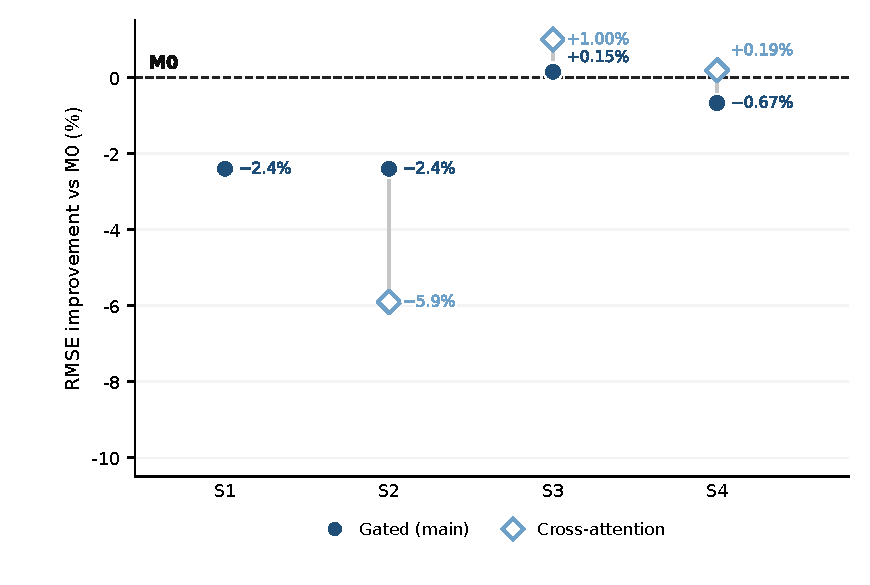
\includegraphics[width=1\linewidth]{../../05_outputs/figures/fig_4_2_deep_rmse_improvement} 

}

\caption{Deep-model RMSE improvement relative to M0. Filled markers denote the prespecified gated specification; hollow markers denote the secondary cross-attention comparison. The dashed line denotes zero improvement relative to M0. Positive values indicate lower RMSE than M0. S1 shows only the finance-only gated specification; no cross-attention result is available because only the finance encoder is active.}\label{fig:deep-rmse}
\end{figure}

Figure \ref{fig:deep-rmse} shows the same RMSE improvements as Table \ref{tab:deep-perf}. In S2, cross-attention is worse than gated fusion. In S3 both models cross M0, and cross-attention records the larger improvement. In S4 only cross-attention is slightly better than M0. Gated S3 is the only prespecified main specification with a positive improvement.

The gated S1 and S2 models record similar RMSE of 4.250 and 4.253, both higher than that of M0. Adding remote sensing therefore provides no descriptive improvement. Neither reported fusion approach reduces RMSE relative to the finance-only Deep model at S2. With shipping included, gated S3 records the lowest RMSE among the gated models at 4.146, improving on M0 by 0.15\%. Gated S4 rises to 4.180, 0.67\% worse than M0, indicating that adding remote sensing to S3 does not provide a further improvement.

On the reported seed-42 run, cross-attention has a higher RMSE than gated fusion at S2, at 4.396 compared with 4.253, but lower RMSEs at S3 and S4. Cross-attention records RMSEs of 4.110 and 4.144 at S3 and S4, corresponding to RMSE improvements of 1.00\% and 0.19\%. These results are therefore reported only as descriptive secondary comparisons and do not provide evidence that cross-attention is superior.

Overall, the Deep family performs better than the Flat family, although most Deep specifications still do not outperform M0. For RQ1, shipping provides the clearest improvement. S3 achieves the best performance under both gated fusion and cross-attention, and both models outperform M0 in the reported run. Remote sensing provides little additional value. It does not improve the finance-only model at S2 and weakens the gated model when added to shipping at S4.

\section{Flat versus Deep}\label{results-flat-deep}

Table \ref{tab:flat-deep} compares the main Deep model with both Flat models within each feature set. The feature-set category, forecast dates and evaluation sample are held constant. The main Deep pathway uses the finance-only Deep model at S1 and gated fusion at S2--S4.

\begin{longtable}[]{@{}
  >{\raggedright\arraybackslash}p{(\linewidth - 10\tabcolsep) * \real{0.1549}}
  >{\raggedright\arraybackslash}p{(\linewidth - 10\tabcolsep) * \real{0.1831}}
  >{\raggedright\arraybackslash}p{(\linewidth - 10\tabcolsep) * \real{0.1268}}
  >{\raggedright\arraybackslash}p{(\linewidth - 10\tabcolsep) * \real{0.1831}}
  >{\raggedright\arraybackslash}p{(\linewidth - 10\tabcolsep) * \real{0.1268}}
  >{\raggedright\arraybackslash}p{(\linewidth - 10\tabcolsep) * \real{0.2254}}@{}}
\caption{\label{tab:flat-deep} Matched Flat--Deep comparisons by feature set (\(n = 257\)).}\tabularnewline
\toprule\noalign{}
\begin{minipage}[b]{\linewidth}\raggedright
Feature set
\end{minipage} & \begin{minipage}[b]{\linewidth}\raggedright
Flat model
\end{minipage} & \begin{minipage}[b]{\linewidth}\raggedright
Flat RMSE
\end{minipage} & \begin{minipage}[b]{\linewidth}\raggedright
Deep model
\end{minipage} & \begin{minipage}[b]{\linewidth}\raggedright
Deep RMSE
\end{minipage} & \begin{minipage}[b]{\linewidth}\raggedright
Deep vs Flat (\%)
\end{minipage} \\
\midrule\noalign{}
\endfirsthead
\toprule\noalign{}
\begin{minipage}[b]{\linewidth}\raggedright
Feature set
\end{minipage} & \begin{minipage}[b]{\linewidth}\raggedright
Flat model
\end{minipage} & \begin{minipage}[b]{\linewidth}\raggedright
Flat RMSE
\end{minipage} & \begin{minipage}[b]{\linewidth}\raggedright
Deep model
\end{minipage} & \begin{minipage}[b]{\linewidth}\raggedright
Deep RMSE
\end{minipage} & \begin{minipage}[b]{\linewidth}\raggedright
Deep vs Flat (\%)
\end{minipage} \\
\midrule\noalign{}
\endhead
\bottomrule\noalign{}
\endlastfoot
S1 & Ridge & 4.256 & M1--Deep & 4.250 & +0.15\% \\
S1 & M1--Flat--XGB & 4.368 & M1--Deep & 4.250 & +2.71\% \\
S2 & M2--Flat--Ridge & 4.414 & M2--Deep--Gated & 4.253 & +3.64\% \\
S2 & M2--Flat--XGB & 4.440 & M2--Deep--Gated & 4.253 & +4.22\% \\
S3 & M3--Flat--Ridge & 4.553 & M3--Deep--Gated & 4.146 & +8.95\% \\
S3 & M3--Flat--XGB & 4.357 & M3--Deep--Gated & 4.146 & +4.85\% \\
S4 & M4--Flat--Ridge & 4.539 & M4--Deep--Gated & 4.180 & +7.90\% \\
S4 & M4--Flat--XGB & 4.412 & M4--Deep--Gated & 4.180 & +5.26\% \\
\end{longtable}

\emph{Note:} Positive values indicate a lower Deep RMSE than the matched Flat model.

\begin{figure}

{\centering 
\includegraphics[width=0.9\linewidth]{../../05_outputs/figures/fig_4_3_flat_vs_deep_slope} 

}

\caption{Change in out-of-sample price RMSE from flat XGBoost to gated Deep models. All results use the common 257-week evaluation sample. The dashed line marks the M0 no-change benchmark. S1 is included as a modelling-path reference, while the modality-matched comparisons relevant to RQ2 are S2–S4.}\label{fig:flat-deep-slope}
\end{figure}

Across all four feature sets, the main Deep model records lower RMSE than both Ridge and XGBoost. The reduction ranges from 0.15\% against Ridge at S1 to 8.95\% against Ridge at S3. At S1 and S2, the main Deep models improve on both Flat learners but remain worse than M0. S3 is the only feature set which has lower RMSE than M0. Although the main Deep S4 model improves substantially over both Flat models, it remains worse than M0 and does not improve on the main Deep S3 model.

Overall, these comparisons show that the main Deep pathway records lower RMSE than both Flat learners across all four feature sets. For RQ2, this provides consistent evidence that modality-aware representation-level modelling performs better than flat feature fusion when using matched modality sets. However, because the Deep and Flat pathways also differ in model architecture and data representation, the improvement cannot be attributed to representation-level fusion alone. Nevertheless, the comparison suggests that how heterogeneous data are organised and represented may affect the extent to which different information is retained and used by the model, and that preserving the distinct structure and characteristics of different data types may be valuable for future research.

\section{Interpretability}\label{results-interp}

Following the eligibility rule in Section \ref{method-interp}, interpretation is reported for the gated Deep model on S3. Table \ref{tab:period-attr} combines period-specific forecast performance, modality-gate weights and absolute SHAP attribution for the 257 forecast origins.

\begin{longtable}[]{@{}
  >{\raggedright\arraybackslash}p{(\linewidth - 14\tabcolsep) * \real{0.1505}}
  >{\raggedright\arraybackslash}p{(\linewidth - 14\tabcolsep) * \real{0.0323}}
  >{\raggedright\arraybackslash}p{(\linewidth - 14\tabcolsep) * \real{0.0538}}
  >{\raggedright\arraybackslash}p{(\linewidth - 14\tabcolsep) * \real{0.2258}}
  >{\raggedright\arraybackslash}p{(\linewidth - 14\tabcolsep) * \real{0.1290}}
  >{\raggedright\arraybackslash}p{(\linewidth - 14\tabcolsep) * \real{0.1398}}
  >{\raggedright\arraybackslash}p{(\linewidth - 14\tabcolsep) * \real{0.1290}}
  >{\raggedright\arraybackslash}p{(\linewidth - 14\tabcolsep) * \real{0.1398}}@{}}
\caption{\label{tab:period-attr} Period-specific performance and attribution for gated Deep S3.}\tabularnewline
\toprule\noalign{}
\begin{minipage}[b]{\linewidth}\raggedright
Period
\end{minipage} & \begin{minipage}[b]{\linewidth}\raggedright
n
\end{minipage} & \begin{minipage}[b]{\linewidth}\raggedright
RMSE
\end{minipage} & \begin{minipage}[b]{\linewidth}\raggedright
Improvement vs M0 (\%)
\end{minipage} & \begin{minipage}[b]{\linewidth}\raggedright
Gate finance
\end{minipage} & \begin{minipage}[b]{\linewidth}\raggedright
Gate shipping
\end{minipage} & \begin{minipage}[b]{\linewidth}\raggedright
SHAP finance
\end{minipage} & \begin{minipage}[b]{\linewidth}\raggedright
SHAP shipping
\end{minipage} \\
\midrule\noalign{}
\endfirsthead
\toprule\noalign{}
\begin{minipage}[b]{\linewidth}\raggedright
Period
\end{minipage} & \begin{minipage}[b]{\linewidth}\raggedright
n
\end{minipage} & \begin{minipage}[b]{\linewidth}\raggedright
RMSE
\end{minipage} & \begin{minipage}[b]{\linewidth}\raggedright
Improvement vs M0 (\%)
\end{minipage} & \begin{minipage}[b]{\linewidth}\raggedright
Gate finance
\end{minipage} & \begin{minipage}[b]{\linewidth}\raggedright
Gate shipping
\end{minipage} & \begin{minipage}[b]{\linewidth}\raggedright
SHAP finance
\end{minipage} & \begin{minipage}[b]{\linewidth}\raggedright
SHAP shipping
\end{minipage} \\
\midrule\noalign{}
\endhead
\bottomrule\noalign{}
\endlastfoot
Full sample & 257 & 4.146 & +0.15\% & 0.558 & 0.442 & 96.8\% & 3.2\% \\
2021 & 50 & 3.014 & −1.98\% & 0.521 & 0.479 & 95.8\% & 4.2\% \\
2022 & 52 & 6.613 & +0.77\% & 0.519 & 0.481 & 96.4\% & 3.6\% \\
2023 & 52 & 3.790 & −0.37\% & 0.481 & 0.519 & 94.8\% & 5.2\% \\
2024 & 52 & 3.083 & −0.79\% & 0.520 & 0.480 & 95.0\% & 5.0\% \\
2025 & 51 & 2.960 & +0.99\% & 0.749 & 0.251 & 99.2\% & 0.8\% \\
Russia--Ukraine & 16 & 8.822 & +1.15\% & 0.536 & 0.464 & 96.5\% & 3.5\% \\
EU oil ban & 16 & 5.059 & −0.21\% & 0.524 & 0.476 & 96.0\% & 4.0\% \\
OPEC+ & 16 & 4.358 & +0.76\% & 0.485 & 0.515 & 95.7\% & 4.3\% \\
Red Sea & 16 & 3.265 & +2.55\% & 0.489 & 0.511 & 94.1\% & 5.9\% \\
\end{longtable}

\emph{Note:} RMSE is evaluated in price levels, while SHAP attributes predicted log returns. Event windows are ±8 weeks.

\begin{figure}

{\centering 
\includegraphics[width=1\linewidth]{../05_outputs/figures/fig_4_3_shap_modality} 

}

\caption{Shipping gate weights and shipping shares of absolute SHAP for the full sample, calendar years and ±8-week event windows, gated Deep S3. Finance values are omitted because they equal 100\% minus the corresponding shipping values. Gate weights and SHAP shares are not interchangeable.}\label{fig:shap-modality}
\end{figure}

Financial inputs dominate absolute SHAP throughout the sample, accounting for 96.8\% of full-sample attribution compared with 3.2\% for shipping. Shipping attribution is relatively higher in 2023--2024 and during the Red Sea window, at between 5.0\% and 5.9\%, but falls to 0.8\% in 2025. Its contribution is therefore small and episodic rather than persistently elevated.

The main-run gate allocates average weights of 55.8\% to finance and 44.2\% to shipping, a substantially more balanced division than the SHAP attribution. Figure \ref{fig:shap-modality} isolates this contrast for shipping: the gate assigns it a representation weight of about 25--52\%, while its realised share of absolute SHAP remains 0.8--5.9\%. The two quantities are not interchangeable; SHAP is therefore used as the primary basis for interpreting RQ3.

At the input-group level, EIA variables provide the largest full-sample contribution at 43.6\%, followed by financial and macroeconomic variables at 31.4\%. All twenty highest-ranked individual features are financial inputs, led by crude production, Cushing stocks and the federal funds rate. No shipping subgroup contributes more than 2.0\% in any reported period, although PortWatch and SAR become modestly more prominent during the Red Sea window.

Within the shipping representation, the highest full-sample node shares belong to Jurong, Hormuz, Suez, the Cape route and Bab el-Mandeb. Jurong and Hormuz lead the rankings from 2021 to 2023, while Suez, Bab el-Mandeb and the Cape route occupy the first three positions in 2024. Figure \ref{fig:node-shap-map} shows this shift for 2022 and 2024, the two calendar years with the largest node-share reallocation. Figure \ref{fig:node-shap-heatmap} tracks the same within-shipping shares through time. During the ±8-week Red Sea window, the largest trailing six-week mean of any node's within-shipping share was 14.0\% (Suez). These shares are normalised within the shipping modality and do not represent each node's share of total-model attribution.

\begin{figure}

{\centering 
\includegraphics[width=1\linewidth]{../../05_outputs/figures/fig_4_4_node_shap_map} 

}

\caption{Node-level shipping SHAP shares for 2022 and 2024, the two calendar years with the largest geographic reallocation of shipping attribution. Halo size scales with the share of shipping attribution (locked scale of 18\%). Other nodes are shown as fixed-size grey dots.}\label{fig:node-shap-map}
\end{figure}



\begin{figure}

{\centering 
\includegraphics[width=1\linewidth]{../../05_outputs/figures/fig_4_5_node_shap_heatmap} 

}

\caption{Trailing six-week mean of each node's share of absolute SHAP within the shipping modality, gated Deep S3. Chokepoint nodes appear above AOI nodes; within each group, nodes are ordered by full-sample within-shipping share (high to low). These shares are normalised within the shipping modality and do not represent each node's share of total-model attribution. The colour scale is locked at 18\%, matching Figure \ref{fig:node-shap-map}. Grey bands mark ±8-week event windows: Russia--Ukraine (24 February 2022), EU oil ban (1 June 2022), OPEC+ (2 April 2023) and Red Sea (19 November 2023). During the Red Sea window, the largest smoothed within-shipping node share was 14.0\% (Suez). Light-grey cells at the start of the sample are undefined trailing means (fewer than six weeks of history).}\label{fig:node-shap-heatmap}
\end{figure}

For RQ3, the model relies predominantly on financial information across all market conditions. Shipping provides a much smaller and more episodic contribution, becoming relatively more important in some periods of market and trade disruption, particularly in 2023--2024 and during the Red Sea event window. Its geographic focus also shifts over time across major ports and chokepoints rather than remaining concentrated in one location. Overall, the results suggest that financial data provide the model's core predictive information, while shipping data act as a supplementary source whose importance increases under particular market conditions.

\section{Robustness}\label{results-robustness}

Table \ref{tab:seed-robust} reports the results of rerunning all Deep specifications with multiple random seeds.

\begin{longtable}[]{@{}
  >{\raggedright\arraybackslash}p{(\linewidth - 8\tabcolsep) * \real{0.0429}}
  >{\raggedright\arraybackslash}p{(\linewidth - 8\tabcolsep) * \real{0.2000}}
  >{\raggedright\arraybackslash}p{(\linewidth - 8\tabcolsep) * \real{0.2857}}
  >{\raggedright\arraybackslash}p{(\linewidth - 8\tabcolsep) * \real{0.2857}}
  >{\raggedright\arraybackslash}p{(\linewidth - 8\tabcolsep) * \real{0.1857}}@{}}
\caption{\label{tab:seed-robust} Random-seed robustness of all Deep specifications (improvement vs M0, \%).}\tabularnewline
\toprule\noalign{}
\begin{minipage}[b]{\linewidth}\raggedright
Set
\end{minipage} & \begin{minipage}[b]{\linewidth}\raggedright
Model
\end{minipage} & \begin{minipage}[b]{\linewidth}\raggedright
Main-run improvement
\end{minipage} & \begin{minipage}[b]{\linewidth}\raggedright
Across-run mean ± SD
\end{minipage} & \begin{minipage}[b]{\linewidth}\raggedright
Positive runs
\end{minipage} \\
\midrule\noalign{}
\endfirsthead
\toprule\noalign{}
\begin{minipage}[b]{\linewidth}\raggedright
Set
\end{minipage} & \begin{minipage}[b]{\linewidth}\raggedright
Model
\end{minipage} & \begin{minipage}[b]{\linewidth}\raggedright
Main-run improvement
\end{minipage} & \begin{minipage}[b]{\linewidth}\raggedright
Across-run mean ± SD
\end{minipage} & \begin{minipage}[b]{\linewidth}\raggedright
Positive runs
\end{minipage} \\
\midrule\noalign{}
\endhead
\bottomrule\noalign{}
\endlastfoot
S1 & M1-Deep & −2.36\% & −1.00\% ± 1.33 & 1/3 \\
S2 & M2-Deep-Gated & −2.43\% & −3.15\% ± 1.67 & 0/3 \\
& M2-Deep-Concat & −2.01\% & −1.79\% ± 0.77 & 0/3 \\
& M2-Deep-XAttn & −5.87\% & −3.57\% ± 2.77 & 0/3 \\
S3 & M3-Deep-Gated & +0.15\% & −0.51\% ± 0.80 & 1/3 \\
& M3-Deep-Concat & −0.22\% & −0.27\% ± 0.35 & 1/3 \\
& M3-Deep-XAttn & +1.00\% & −3.01\% ± 4.07 & 1/3 \\
S4 & M4-Deep-Gated & −0.68\% & −0.91\% ± 0.26 & 0/3 \\
& M4-Deep-Concat & −8.30\% & −3.79\% ± 3.95 & 0/3 \\
& M4-Deep-XAttn & +0.19\% & −1.90\% ± 2.75 & 1/3 \\
\end{longtable}

\emph{Note:} The main-run column is the seed-42 result reported in Tables \ref{tab:deep-perf}--\ref{tab:period-attr}. S1 has no fusion operator. XAttn denotes cross-attention. Individual seeds are shown in Appendix B (Figure \ref{fig:seed-robustness}).

None of the models achieves a positive mean RMSE improvement relative to M0 across runs, and only five of the thirty individual runs are positive. No S2 fusion is positive in any seed. S3 concatenation has the best mean result, but it is still negative at −0.27\%, while the main gated S3 model records −0.51\%. Across seeds the S3 order reverses: concatenation (−0.27\%) remains closest to M0, ahead of gated (−0.51\%) and cross-attention (−3.01\%). Gated S3 also outperforms S1 in only one of the three matched runs. The positive improvements observed in the main run are therefore sensitive to random initialisation. Gated fusion remains the main specification because it supplies modality weights for RQ3, not because it is the more accurate operator. Overall, although the Deep models do not consistently outperform M0, some specifications, particularly S3, show predictive potential and merit further investigation. The better-performing Deep specifications remain broadly close to M0 rather than demonstrating a consistent forecasting advantage.

\chapter{Discussion}\label{discussion}

\section{RQ1 --- Do spatial data help?}\label{discussion-rq1}

RQ1 asked whether remote sensing and shipping add out-of-sample value beyond financial time series. The answer depends on the modelling pathway.

Within the Flat family, no model outperforms the no-change benchmark, consistent with the short-horizon oil-forecasting literature that treats the no-change forecast as a demanding reference (\citeproc{ref-alquist2013}{Alquist, Kilian and Vigfusson, 2013}). Relative to the finance-only S1 specification, remote sensing increases forecast error for both Ridge and XGBoost, while shipping increases error for Ridge but slightly reduces it for XGBoost. The latter result shows that shipping is not uniformly detrimental within the Flat pathway, but the improvement remains insufficient to outperform M0. Overall, simply adding spatial features to Flat models does not produce additional predictive value.

Under the Deep pathway, adding remote sensing to finance in S2 does not improve forecast accuracy over either S1 or M0. By contrast, adding shipping to finance in S3 produces a small positive RMSE improvement relative to M0, making S3 the best-performing specification in the main gated pathway. Extending S3 with remote sensing in S4 does not further reduce forecast error. The secondary cross-attention results show the same ordering across the multimodal specifications, with S3 performing best, followed by S4 and S2. Shipping is therefore the more informative spatial source in this design, while remote sensing contributes little to predictive accuracy. The improvement is notable because the other main modelling specifications fail to beat M0, although the gain remains limited.

Observations of activity across multiple ports and chokepoints appear to be more useful for short-term forecasting than the selected remote-sensing measures from individual sites. The limited value of remote sensing may be due to a mismatch in scale: the satellite data are monthly and local, while Brent is constructed at a weekly frequency.

These findings refine the AIS and satellite literature reviewed in Chapter \ref{literature}. Existing studies often demonstrate that ships and satellites contain information about trade or physical activity (\citeproc{ref-adland2017}{Adland, Jia and Strandenes, 2017}; \citeproc{ref-yan2020}{Yan \emph{et al.}, 2020}; \citeproc{ref-hao2023}{Hao and Wang, 2023}), but less often ask whether those signals improve one-week-ahead Brent forecasts relative to both a financial baseline and M0. The present results distinguish informational content from predictive value. The ability to measure trade or industrial activity does not necessarily produce a forecast improvement against a demanding weekly benchmark.

\section{RQ2 --- Does representation-level fusion beat flat fusion?}\label{discussion-rq2}

RQ2 asked whether representation-level Deep modelling outperforms flat feature fusion under the same information sets and evaluation protocol. Across the matched multimodal sets S2--S4, the main Deep pathway records lower RMSE than the Flat learners. The largest differences appear in S3 and S4, both of which include shipping data. The results therefore show that the Deep pathway outperforms early feature concatenation under the current framework. However, outperforming the Flat models does not necessarily mean outperforming the no-change benchmark.

Early-fusion approaches combine heterogeneous predictors within a single feature space, whereas multimodal models retain separate representations before fusion (\citeproc{ref-arevalo2017}{Arevalo \emph{et al.}, 2017}; \citeproc{ref-gohari2024}{Gohari \emph{et al.}, 2024}). This study extends the comparison to weekly Brent forecasting. The larger Deep advantage in S3 and S4 provides further support for the value of representation-level modelling. From a spatial perspective, representation-level modelling may be particularly useful for observations distributed across networks of ports and chokepoints. Spatial relationships among shipping nodes can provide additional structural information. By contrast, treating these observations as independent tabular features does not explicitly preserve these relationships.

However, the comparisons in this study evaluate complete modelling pathways, including their encoders and fusion strategies. They therefore support the overall Deep approach but do not identify the preservation of network structure or any individual fusion operator as the cause of its better performance.

\section{RQ3 --- What does the model rely on when value exists?}\label{discussion-rq3}

RQ3 asked how the model uses information when a specification improves on the benchmark. The gate and SHAP results show that the internally learned weights assigned to each data source do not directly correspond to their contributions to the model output. The forecast still relies mainly on financial and EIA information, while shipping provides incremental predictive information beyond the financial inputs. Although shipping has a relatively small SHAP contribution, gated Deep S3 still records a small RMSE improvement relative to M0. This suggests that a modality can add predictive value even if it accounts for only a small share of the model's output.

This incremental role also varies with the type of disruption. Shipping becomes relatively more important during the Red Sea period, while financial inputs remain more prominent during the Russia--Ukraine window. This difference is consistent with the nature of the two disruptions. Transport-specific disruptions may increase the relevance of maritime activity, whereas broader geopolitical shocks may affect Brent through several channels, including supply expectations, inventories and financial markets. The spatial pattern supports this interpretation. The model's focus shifts from Jurong and Hormuz in earlier years to Suez, Bab el-Mandeb and the Cape route in 2024. This broadly matches the disruption and rerouting around the Red Sea. However, no single location dominates during this period. The model therefore appears to respond to changes in the geographic pattern of shipping activity rather than consistently relying on the same chokepoints.

Attention and gate weights describe operations within fitted models rather than causal relationships. SHAP attributes the model's Brent predictions rather than explaining the causes of price movements. Therefore, the temporal and spatial analysis can highlight periods and transport corridors that deserve further study, but it should not be interpreted as a direct signal for policy action.

\section{Implications}\label{discussion-implications}

Model choice should be aligned with the structure of the input data. Relational data, such as shipping networks, capture relationships among observations that may carry useful information. Preserving this structure before fusion may therefore be more appropriate than direct feature concatenation. More generally, new data sources should be evaluated under a common out-of-sample framework. Their value should be compared both against a model using only established predictors and against a simple benchmark forecast. The first comparison tests whether the new data add information beyond conventional inputs, while the second tests whether the full modelling system improves on a basic forecasting rule.

These models provide diagnostic rather than causal insight into oil prices. They show which information is useful for one-week-ahead prediction and help identify periods or parts of the supply network that deserve further analysis. However, they do not explain the mechanisms that cause oil prices to move. Their main value is therefore to integrate and assess predictive information from different sources, thereby supporting further analysis of oil-market conditions.

Spatial data should be assessed according to how well their scale, frequency and structure match the analytical task. Remote sensing describes conditions at selected facilities, so it may be more suitable for monitoring facility activity or regional production. Shipping data capture flows across connected ports, chokepoints and routes, and therefore better reflect disruptions and adjustments across the global oil supply network. Better observation of such physical activity may be useful for applications such as energy-security monitoring, trade planning and inflation-sensitive fiscal management, but it does not necessarily improve one-week-ahead Brent forecasts. More broadly, this study suggests that the value of a data source depends on the task for which it is used. A data source may be useful for forecasting, monitoring, explanation or risk detection, without being equally useful for all of them. In particular, monitoring value and predictive value should be assessed separately, since data that effectively capture physical activity or market stress may not necessarily improve forecasts.

\section{Limitations}\label{discussion-limitations}

The sample size in this study is limited because of the availability of the different data sources. The evaluation contains only 257 rolling out-of-sample forecasts. Deep S3 improves only slightly over M0, and the improvement is concentrated in certain periods and event windows. This suggests that its predictive value is limited and conditional rather than consistently stable. The findings are specific to one-week-ahead Brent forecasting and should not be generalised to other forecast horizons.

The study applies a range of methods to reduce information leakage, including publication lags and as-of alignment, but limitations in data availability and preprocessing remain. The study uses revised historical series rather than real-time vintages and therefore does not fully reproduce the information available at each forecast origin. Monthly GFW and remote-sensing inputs are carried forward weekly between releases, limiting their ability to capture short-lived changes. Some variables are also indirect proxies, while preprocessing and representation choices such as missing-value treatment and the use of fixed Prithvi-EO-2.0 embeddings introduce additional assumptions. The observed model performance therefore cannot be attributed to the source data alone.

The spatial findings are conditional on the coverage and construction of a purposively selected network of eleven sites and six chokepoints. The site sample is weighted toward Gulf export and transshipment nodes and Asian import and refining hubs, although it also includes Rotterdam and Houston. No site-level AOIs are located in Russia, West Africa or Latin America, although the Panama Canal is included as a chokepoint. These omissions partly reflect constraints on consistent cross-source data availability and satellite observability over the full study period, although using observability as a site-selection criterion may itself introduce geographic bias. The importance assigned to individual nodes by the model therefore reflects dependence within this constructed network rather than a comprehensive ranking of global oil infrastructure.

The comparison between the Flat and Deep families evaluates differences between complete modelling pathways rather than differences in any single model component. The two pathways differ in model class, data representation and fusion approach. For example, the Deep shipping pathway additionally introduces an explicit graph structure. Therefore, the observed performance differences cannot be clearly attributed to any single model architecture or to the gated-fusion mechanism itself.

\section{Future research}\label{discussion-future}

Future research should test whether the value of shipping data remains stable over longer periods and across a wider oil-transport network. A longer-term evaluation could use archived data releases and include additional regions such as Russian Baltic and Black Sea ports, West African loading areas and Latin American exporters. This would provide evidence from a longer time period and broader geographic coverage. Where AIS data are incomplete, SAR-based vessel detection could help capture vessel activity not visible in AIS data, including dark-fleet activity.

Future research should test the transferability of this framework by applying it to other forecasting tasks and markets. The same Flat--Deep comparison could be applied to other energy commodities and markets, such as WTI crude oil, LNG and natural gas. It could also be extended to grain and metal markets to test whether modelling network structure remains useful outside the energy sector. Remote sensing should be evaluated for targets that better match its spatial and temporal scale, such as facility activity, regional production or longer-term price movements. Where possible, future studies should also compare Flat and Deep remote-sensing models using the same underlying inputs. This would make it easier to separate the effect of model architecture from differences in data representation.

Future research should evaluate the practical value of the forecasts. For public-sector applications, probabilistic forecasts and scenario ranges could be compared with existing financial and EIA monitoring. This would help assess whether shipping information improves the timing and focus of energy-security monitoring, trade planning or inflation-sensitive budgeting. Evaluating policy actions such as strategic reserve releases, sanctions or fiscal responses would require more than forecasting alone. Forecasting models would need to be combined with causal or decision-analysis methods to estimate how these actions affect prices, supply and policy costs. Model attribution should therefore be used as a diagnostic tool rather than as an automatic policy signal.

\chapter{Conclusion}\label{conclusion}

Short-horizon oil-price surprises affect hedging, budgeting and market-risk decisions, yet weekly Brent forecasts remain difficult to improve on a simple no-change rule. Using weekly data from 2019 to 2025, this dissertation examined whether satellite remote sensing and maritime shipping add predictive information beyond conventional financial and physical-market indicators, and whether preserving the structure of each data type improves on flat feature fusion. Under a common rolling out-of-sample design, each data addition was compared with both a finance-only model and the no-change benchmark, separating incremental contribution from overall forecast performance.

The results show that additional data and model complexity do not automatically produce better forecasts. Remote sensing added no forecast value, whether introduced alone or on top of shipping. Shipping was more useful, but no Flat model outperformed the no-change benchmark. Among the main specifications, only the modality-aware finance-plus-shipping model achieved a small improvement. Across matched information sets, modality-aware models generally produced lower errors than flat fusion. This shows that preserving data structure can improve relative performance without guaranteeing forecasts that outperform the benchmark. Model diagnostics indicated that predictions remained led by financial and EIA information, while shipping made a smaller contribution that varied across disruption periods and locations in the transport network. These patterns show how the model used the available information but do not identify the causes of oil-price movements.

The main contribution is a clearer standard for deciding when alternative spatial data constitute forecast evidence. Their value depends on whether their scale, frequency and structure match the forecasting target, and whether they improve on both conventional information and a simple forecasting rule. Remote sensing of local facility conditions may be better suited to facility or regional monitoring, while shipping observations can complement monitoring of network-wide disruption and rerouting. For energy-security monitoring, trade planning and inflation-sensitive budgeting, financial and EIA indicators should therefore remain the core, with spatial data providing additional context rather than stand-alone policy signals. Better observation of physical stress is not the same as better short-horizon price prediction.

Future research should test the transferability of these findings using longer real-time histories, broader transport networks and stricter like-for-like model comparisons, alongside economic and policy evaluation. Rather than identifying a universally superior model or data source, this study shows that the predictive value of alternative data depends on alignment with the target, how the data are represented and whether improvements hold against credible benchmarks.

\chapter*{References}\label{references}

\protect\phantomsection\label{refs}
\begin{CSLReferences}{0}{1}
\bibitem[\citeproctext]{ref-adland2017}
Adland, R., Jia, H. and Strandenes, S.P. (2017) {``Are {AIS}-based trade volume estimates reliable? The case of crude oil exports,''} \emph{Maritime Policy \& Management}, 44(5), pp. 657--665. Available at: \url{https://doi.org/10.1080/03088839.2017.1309470}.

\bibitem[\citeproctext]{ref-alquist2013}
Alquist, R., Kilian, L. and Vigfusson, R.J. (2013) {``Forecasting the price of oil,''} in G. Elliott and A. Timmermann (eds.) \emph{Handbook of economic forecasting}. Amsterdam: Elsevier, pp. 427--507. Available at: \url{https://doi.org/10.1016/B978-0-444-53683-9.00008-6}.

\bibitem[\citeproctext]{ref-arevalo2017}
Arevalo, J. \emph{et al.} (2017) {``Gated multimodal units for information fusion,''} \emph{{ICLR} 2017 workshop track}. Toulon, France. Available at: \url{https://openreview.net/forum?id=S12_nquOe} (Accessed: July 1, 2026).

\bibitem[\citeproctext]{ref-arslanalp2026}
Arslanalp, S. \emph{et al.} (2026) \emph{Nowcasting country-level trade estimates using {IMF} {PortWatch}}. IMF Working Paper WP/26/99. Washington, DC: International Monetary Fund. Available at: \url{https://doi.org/10.5089/9798229046893.001}.

\bibitem[\citeproctext]{ref-arslanalp2019}
Arslanalp, S., Marini, M. and Tumbarello, P. (2019) \emph{Big data on vessel traffic: Nowcasting trade flows in real time}. IMF Working Paper WP/19/275. Washington, DC: International Monetary Fund. Available at: \url{https://www.imf.org/en/publications/wp/issues/2019/12/13/big-data-on-vessel-traffic-nowcasting-trade-flows-in-real-time-48837} (Accessed: July 1, 2026).

\bibitem[\citeproctext]{ref-bai2018}
Bai, S., Kolter, J.Z. and Koltun, V. (2018) {``An empirical evaluation of generic convolutional and recurrent networks for sequence modeling.''} Available at: \url{https://arxiv.org/abs/1803.01271} (Accessed: August 3, 2026).

\bibitem[\citeproctext]{ref-baltrusaitis2019}
Baltrušaitis, T., Ahuja, C. and Morency, L.-P. (2019) {``Multimodal machine learning: A survey and taxonomy,''} \emph{IEEE Transactions on Pattern Analysis and Machine Intelligence}, 41(2), pp. 423--443. Available at: \url{https://doi.org/10.1109/TPAMI.2018.2798607}.

\bibitem[\citeproctext]{ref-baumeister2015}
Baumeister, C. and Kilian, L. (2015) {``Forecasting the real price of oil in a changing world: A forecast combination approach,''} \emph{Journal of Business \& Economic Statistics}, 33(3), pp. 338--351. Available at: \url{https://doi.org/10.1080/07350015.2014.949342}.

\bibitem[\citeproctext]{ref-bricongne2026}
Bricongne, J.-C. \emph{et al.} (2026) \emph{Can satellites predict oil demand?} ECB Working Paper Series 3198. Frankfurt am Main: European Central Bank. Available at: \url{https://www.ecb.europa.eu/pub/pdf/scpwps/ecb.wp3198~e3858c52a3.en.pdf} (Accessed: July 1, 2026).

\bibitem[\citeproctext]{ref-che2018}
Che, Z. \emph{et al.} (2018) {``Recurrent neural networks for multivariate time series with missing values,''} \emph{Scientific Reports}, 8, p. 6085. Available at: \url{https://doi.org/10.1038/s41598-018-24271-9}.

\bibitem[\citeproctext]{ref-chen2016}
Chen, T. and Guestrin, C. (2016) {``{XGBoost}: A scalable tree boosting system,''} \emph{Proceedings of the 22nd {ACM} {SIGKDD} international conference on knowledge discovery and data mining}. New York, NY: Association for Computing Machinery, pp. 785--794. Available at: \url{https://doi.org/10.1145/2939672.2939785}.

\bibitem[\citeproctext]{ref-cong2022}
Cong, Y. \emph{et al.} (2022) {``{SatMAE}: Pre-training transformers for temporal and multi-spectral satellite imagery,''} \emph{Advances in neural information processing systems}. Red Hook, NY: Curran Associates, pp. 197--211.

\bibitem[\citeproctext]{ref-costa2021}
Costa, A.B.R. \emph{et al.} (2021) {``Machine learning and oil price point and density forecasting,''} \emph{Energy Economics}, 102, p. 105494. Available at: \url{https://doi.org/10.1016/j.eneco.2021.105494}.

\bibitem[\citeproctext]{ref-foroutan2024}
Foroutan, P. and Lahmiri, S. (2024) {``Deep learning systems for forecasting the prices of crude oil and precious metals,''} \emph{Financial Innovation}, 10, p. 111. Available at: \url{https://doi.org/10.1186/s40854-024-00637-z}.

\bibitem[\citeproctext]{ref-fuller2023}
Fuller, A., Millard, K. and Green, J.R. (2023) {``{CROMA}: Remote sensing representations with contrastive radar-optical masked autoencoders,''} \emph{Advances in neural information processing systems}. Red Hook, NY: Curran Associates, pp. 5506--5538.

\bibitem[\citeproctext]{ref-gohari2024}
Gohari, H.E. \emph{et al.} (2024) {``Modality-aware transformer for financial time series forecasting,''} \emph{Proceedings of the 5th {ACM} international conference on {AI} in finance ({ICAIF} '24)}. New York, NY: Association for Computing Machinery, pp. 677--685. Available at: \url{https://doi.org/10.1145/3677052.3698654}.

\bibitem[\citeproctext]{ref-hao2023}
Hao, X. and Wang, Y. (2023) {``Cloud cover and expected oil returns,''} \emph{Humanities and Social Sciences Communications}, 10, p. 605. Available at: \url{https://doi.org/10.1057/s41599-023-02128-5}.

\bibitem[\citeproctext]{ref-hoerl1970}
Hoerl, A.E. and Kennard, R.W. (1970) {``Ridge regression: Biased estimation for nonorthogonal problems,''} \emph{Technometrics}, 12(1), pp. 55--67. Available at: \url{https://doi.org/10.1080/00401706.1970.10488634}.

\bibitem[\citeproctext]{ref-jain2019}
Jain, S. and Wallace, B.C. (2019) {``Attention is not explanation,''} \emph{Proceedings of the 2019 conference of the north american chapter of the association for computational linguistics: Human language technologies}. Stroudsburg, PA: Association for Computational Linguistics, pp. 3543--3556. Available at: \url{https://doi.org/10.18653/v1/N19-1357}.

\bibitem[\citeproctext]{ref-jung2026}
Jung, Y. (2026) {``Watching trade from space: Nowcasting and spatial extrapolation of port-level maritime trade using satellite imagery.''} Available at: \url{https://arxiv.org/abs/2604.15444} (Accessed: July 1, 2026).

\bibitem[\citeproctext]{ref-kilian2009}
Kilian, L. (2009) {``Not all oil price shocks are alike: Disentangling demand and supply shocks in the crude oil market,''} \emph{American Economic Review}, 99(3), pp. 1053--1069. Available at: \url{https://doi.org/10.1257/aer.99.3.1053}.

\bibitem[\citeproctext]{ref-liang2022}
Liang, M. \emph{et al.} (2022) {``Fine-grained vessel traffic flow prediction with a spatio-temporal multigraph convolutional network,''} \emph{IEEE Transactions on Intelligent Transportation Systems}, 23(12), pp. 23694--23707. Available at: \url{https://doi.org/10.1109/TITS.2022.3199160}.

\bibitem[\citeproctext]{ref-lundberg2017}
Lundberg, S.M. and Lee, S.-I. (2017) {``A unified approach to interpreting model predictions,''} \emph{Advances in neural information processing systems}. Red Hook, NY: Curran Associates, pp. 4765--4774. Available at: \url{https://papers.nips.cc/paper/7062-a-unified-approach-to-interpreting-model-predictions} (Accessed: July 1, 2026).

\bibitem[\citeproctext]{ref-ma2022}
Ma, M. \emph{et al.} (2022) {``Are multimodal transformers robust to missing modality?''} \emph{Proceedings of the {IEEE}/{CVF} conference on computer vision and pattern recognition ({CVPR})}. Piscataway, NJ: IEEE, pp. 18177--18186. Available at: \url{https://doi.org/10.1109/CVPR52688.2022.01764}.

\bibitem[\citeproctext]{ref-mi2022}
Mi, J.J. \emph{et al.} (2022) {``The impact of the crude oil price on tankers' port-call features: Mining the information in automatic identification system,''} \emph{Journal of Marine Science and Engineering}, 10(10), p. 1559. Available at: \url{https://doi.org/10.3390/jmse10101559}.

\bibitem[\citeproctext]{ref-mi2023}
Mi, J.J. \emph{et al.} (2023) {``The nonlinear relationship between oil prices and the number of tankers' port calls: Evidence from {AIS} data,''} \emph{Procedia Computer Science}, 221, pp. 870--877. Available at: \url{https://doi.org/10.1016/j.procs.2023.08.063}.

\bibitem[\citeproctext]{ref-neverova2016}
Neverova, N. \emph{et al.} (2016) {``{ModDrop}: Adaptive multi-modal gesture recognition,''} \emph{IEEE Transactions on Pattern Analysis and Machine Intelligence}, 38(8), pp. 1692--1706. Available at: \url{https://doi.org/10.1109/TPAMI.2015.2461544}.

\bibitem[\citeproctext]{ref-ouyang2022}
Ouyang, Q. \emph{et al.} (2022) {``Long short-term memory and graph convolution network for forecasting the crude oil traffic flow,''} \emph{IEEE Access}, 10, pp. 18922--18932. Available at: \url{https://doi.org/10.1109/ACCESS.2022.3150852}.

\bibitem[\citeproctext]{ref-paolo2024}
Paolo, F.S. \emph{et al.} (2024) {``Satellite mapping reveals extensive industrial activity at sea,''} \emph{Nature}, 625, pp. 85--91. Available at: \url{https://doi.org/10.1038/s41586-023-06825-8}.

\bibitem[\citeproctext]{ref-polinov2022}
Polinov, S., Bookman, R. and Levin, N. (2022) {``A global assessment of night lights as an indicator for shipping activity in anchorage areas,''} \emph{Remote Sensing}, 14(5), p. 1079. Available at: \url{https://doi.org/10.3390/rs14051079}.

\bibitem[\citeproctext]{ref-shukla2021}
Shukla, S.N. and Marlin, B.M. (2021) {``Multi-time attention networks for irregularly sampled time series,''} \emph{International conference on learning representations ({ICLR} 2021)}. Available at: \url{https://openreview.net/forum?id=4c0J6lwQ4} (Accessed: July 1, 2026).

\bibitem[\citeproctext]{ref-simsek2024}
Simsek, A.I. \emph{et al.} (2024) {``A novel approach to predict {WTI} crude spot oil price: {LSTM}-based feature extraction with {Xgboost} regressor,''} \emph{Energy}, 309, p. 133102. Available at: \url{https://doi.org/10.1016/j.energy.2024.133102}.

\bibitem[\citeproctext]{ref-szwarcman2026}
{Szwarcman, D. \emph{et al.}} (2026) {``Prithvi-{EO}-2.0: A versatile multitemporal foundation model for earth observation applications,''} \emph{IEEE Transactions on Geoscience and Remote Sensing}, 64, p. 4400120. Available at: \url{https://doi.org/10.1109/TGRS.2025.3642610}.

\bibitem[\citeproctext]{ref-eia2014}
U.S. Energy Information Administration (2014) {``Benchmarks play an important role in pricing crude oil.''} \emph{Today in Energy}. Available at: \url{https://www.eia.gov/todayinenergy/detail.php?id=18571} (Accessed: August 11, 2026).

\bibitem[\citeproctext]{ref-velickovic2018}
Veličković, P. \emph{et al.} (2018) {``Graph attention networks,''} \emph{International conference on learning representations ({ICLR} 2018)}. Vancouver, Canada. Available at: \url{https://openreview.net/forum?id=rJXMpikCZ} (Accessed: August 3, 2026).

\bibitem[\citeproctext]{ref-wang2019}
Wang, T. \emph{et al.} (2019) {``Estimating the volume of oil tanks based on high-resolution remote sensing images,''} \emph{Remote Sensing}, 11(7), p. 793. Available at: \url{https://doi.org/10.3390/rs11070793}.

\bibitem[\citeproctext]{ref-wittner2020}
Wittner, M. (2020) {``Global crude benchmarks: {Brent} sets the standard.''} Intercontinental Exchange. Available at: \url{https://www.ice.com/global-crude-benchmarks-brent-sets-the-standard} (Accessed: August 11, 2026).

\bibitem[\citeproctext]{ref-yan2020}
Yan, Z. \emph{et al.} (2020) {``Analysis of global marine oil trade based on automatic identification system ({AIS}) data,''} \emph{Journal of Transport Geography}, 83, p. 102637. Available at: \url{https://doi.org/10.1016/j.jtrangeo.2020.102637}.

\bibitem[\citeproctext]{ref-yilmaz2026}
Yılmaz, T.E. and Zehir, C. (2026) {``Strategic risk based forecasting of {Brent} crude oil prices: A comparative analysis of econometric and machine learning models,''} \emph{Entropy}, 28(5), p. 539. Available at: \url{https://doi.org/10.3390/e28050539}.

\bibitem[\citeproctext]{ref-zhao2022}
Zhao, C. \emph{et al.} (2022) {``Spatiotemporal dynamic network for regional maritime vessel flow prediction amid {COVID}-19,''} \emph{Transport Policy}, 129, pp. 78--89. Available at: \url{https://doi.org/10.1016/j.tranpol.2022.09.029}.

\bibitem[\citeproctext]{ref-zhao2023}
Zhao, G., Xue, M. and Cheng, L. (2023) {``A new hybrid model for multi-step {WTI} futures price forecasting based on self-attention mechanism and spatial--temporal graph neural network,''} \emph{Resources Policy}, 85, p. 103956. Available at: \url{https://doi.org/10.1016/j.resourpol.2023.103956}.

\end{CSLReferences}

\appendix
% Appendix TOC: chapter-level entries only (Appendix A/B/C/D), no A.1 / A.1.1 etc.
\addtocontents{toc}{\protect\setcounter{tocdepth}{0}}

\chapter*{Appendix A --- Data: variable dictionary, AOI/chokepoint lists, lags, graph edges}\label{appendix-a-data-variable-dictionary-aoichokepoint-lists-lags-graph-edges}
\addcontentsline{toc}{chapter}{Appendix A --- Data: variable dictionary, AOI/chokepoint lists, lags, graph edges}

\begin{quote}
Merged weekly matrix \texttt{weekly\_feature\_matrix.csv} = 365 weeks × 263 columns
(2019-01-04 → 2025-12-26): 31 M1 + 55 M2 + 164 M3 + 11 masks + 2 targets.
Per-variable literature/industry sourcing is in the modality data dictionaries
(\texttt{03\_data/processed/M\{1,2,3\}/*\_data\_dictionary.md}); this appendix consolidates
the model-facing dictionary, the site lists, the publication lags and the
shipping-graph edge construction.
\end{quote}

These column counts are the data blocks assembled into information sets
S1--S4 (Table \ref{tab:info-sets}). M0 is the no-change benchmark and has no predictor
matrix of its own.

\begin{center}\rule{0.5\linewidth}{0.5pt}\end{center}

\section{A.1 Variable dictionary (M1--M4)}\label{a.1-variable-dictionary-m1m4}

\subsection{A.1.1 M1 --- Finance / macro (31)}\label{a.1.1-m1-finance-macro-31}

M1 is the finance--macro block shared by every information set except M0.
Daily series enter as the Friday last value. Log returns are ln(Pₜ/Pₜ₋₁)
and are not multiplied by 100. Publication lags are in A.3.

\textbf{Prices \& derived (5)}

{\def\LTcaptype{none} % do not increment counter
\begin{longtable}[]{@{}lll@{}}
\toprule\noalign{}
Variable & Meaning & Source \\
\midrule\noalign{}
\endhead
\bottomrule\noalign{}
\endlastfoot
\texttt{brent\_price} & Brent spot (USD/bbl) & EIA \\
\texttt{wti\_price} & WTI Cushing spot (USD/bbl) & EIA \\
\texttt{brent\_log\_return} & Brent weekly log return & derived \\
\texttt{wti\_log\_return} & WTI weekly log return & derived \\
\texttt{brent\_wti\_spread} & Brent − WTI (USD/bbl) & derived \\
\end{longtable}
}

\textbf{EIA WPSR fundamentals (12)}

{\def\LTcaptype{none} % do not increment counter
\begin{longtable}[]{@{}
  >{\raggedright\arraybackslash}p{(\linewidth - 4\tabcolsep) * \real{0.3333}}
  >{\raggedright\arraybackslash}p{(\linewidth - 4\tabcolsep) * \real{0.3333}}
  >{\raggedright\arraybackslash}p{(\linewidth - 4\tabcolsep) * \real{0.3333}}@{}}
\toprule\noalign{}
\begin{minipage}[b]{\linewidth}\raggedright
Variable
\end{minipage} & \begin{minipage}[b]{\linewidth}\raggedright
Meaning
\end{minipage} & \begin{minipage}[b]{\linewidth}\raggedright
Unit
\end{minipage} \\
\midrule\noalign{}
\endhead
\bottomrule\noalign{}
\endlastfoot
\texttt{crude\_stocks\_excl\_spr} & commercial crude stocks excl. SPR & thousand barrels \\
\texttt{cushing\_stocks} & Cushing crude stocks & thousand barrels \\
\texttt{crude\_production} & U.S. crude production & thousand bbl/d \\
\texttt{crude\_imports} & crude imports & thousand bbl/d \\
\texttt{crude\_exports} & crude exports & thousand bbl/d \\
\texttt{refinery\_crude\_input} & refinery crude input & thousand bbl/d \\
\texttt{refinery\_utilisation} & refinery utilisation & \% \\
\texttt{gasoline\_supplied} & gasoline product supplied & thousand bbl/d \\
\texttt{distillate\_supplied} & distillate product supplied & thousand bbl/d \\
\texttt{jet\_fuel\_supplied} & jet-fuel product supplied & thousand bbl/d \\
\texttt{crude\_stocks\_change} & weekly change in commercial stocks & thousand barrels \\
\texttt{cushing\_stocks\_change} & weekly change in Cushing stocks & thousand barrels \\
\end{longtable}
}

\textbf{Macro-financial (5)}

{\def\LTcaptype{none} % do not increment counter
\begin{longtable}[]{@{}lll@{}}
\toprule\noalign{}
Variable & Meaning & Source \\
\midrule\noalign{}
\endhead
\bottomrule\noalign{}
\endlastfoot
\texttt{vix} & CBOE equity-volatility index & FRED VIXCLS \\
\texttt{dollar\_index} & broad nominal USD index & FRED DTWEXBGS \\
\texttt{treasury\_10y} & 10-year Treasury yield & FRED DGS10 \\
\texttt{fed\_funds\_rate} & effective federal funds rate & FRED DFF \\
\texttt{sp500\_log\_return} & S\&P 500 weekly log return & Yahoo \^{}GSPC \\
\end{longtable}
}

\textbf{Derived market/macro (9)}

{\def\LTcaptype{none} % do not increment counter
\begin{longtable}[]{@{}
  >{\raggedright\arraybackslash}p{(\linewidth - 4\tabcolsep) * \real{0.3333}}
  >{\raggedright\arraybackslash}p{(\linewidth - 4\tabcolsep) * \real{0.3333}}
  >{\raggedright\arraybackslash}p{(\linewidth - 4\tabcolsep) * \real{0.3333}}@{}}
\toprule\noalign{}
\begin{minipage}[b]{\linewidth}\raggedright
Variable
\end{minipage} & \begin{minipage}[b]{\linewidth}\raggedright
Meaning
\end{minipage} & \begin{minipage}[b]{\linewidth}\raggedright
Source
\end{minipage} \\
\midrule\noalign{}
\endhead
\bottomrule\noalign{}
\endlastfoot
\texttt{ovx} & CBOE crude-oil volatility index & Yahoo \^{}OVX \\
\texttt{gpr} & geopolitical-risk index (weekly mean of daily GPRD) & Caldara--Iacoviello \\
\texttt{gold\_return} & gold weekly log return & FRED / Yahoo GC=F \\
\texttt{global\_econ\_activity} & Kilian real economic activity (REA) & Dallas Fed IGREA \\
\texttt{nonoil\_industrial\_commodity} & non-fuel industrial materials price index & IMF PINDUINDEXM (FRED) \\
\texttt{brent\_f1\_spot\_log\_basis} & front-month futures − spot log basis & Yahoo BZ=F vs EIA spot \\
\texttt{brent\_roll\_week} & front-month roll-week dummy \{0,1\} & calendar-derived \\
\texttt{cadusd\_log\_return} & CAD/USD weekly log return & Yahoo CADUSD=X \\
\texttt{dgs10\_change} & weekly change in \texttt{treasury\_10y} & derived \\
\end{longtable}
}

\texttt{brent\_f1\_spot\_log\_basis} = ln(BZ=F) − ln(\texttt{brent\_price}); the futures leg is not back-adjusted, so \texttt{brent\_roll\_week} flags the calendar week of the roll.

\subsection{A.1.2 M2 --- Remote sensing (55 = 5 indices × 11 AOI)}\label{a.1.2-m2-remote-sensing-55-5-indices-11-aoi}

Naming \texttt{\{index\}\_anom\_\{AOI\}}; \texttt{anom} = within-site deseasonalised z-score
(expanding, past-only). Raw \texttt{level} and staleness/mask columns are not modelled.

{\def\LTcaptype{none} % do not increment counter
\begin{longtable}[]{@{}
  >{\raggedright\arraybackslash}p{(\linewidth - 6\tabcolsep) * \real{0.2500}}
  >{\raggedright\arraybackslash}p{(\linewidth - 6\tabcolsep) * \real{0.2500}}
  >{\raggedright\arraybackslash}p{(\linewidth - 6\tabcolsep) * \real{0.2500}}
  >{\raggedright\arraybackslash}p{(\linewidth - 6\tabcolsep) * \real{0.2500}}@{}}
\toprule\noalign{}
\begin{minipage}[b]{\linewidth}\raggedright
Index
\end{minipage} & \begin{minipage}[b]{\linewidth}\raggedright
Meaning
\end{minipage} & \begin{minipage}[b]{\linewidth}\raggedright
Formula
\end{minipage} & \begin{minipage}[b]{\linewidth}\raggedright
Source
\end{minipage} \\
\midrule\noalign{}
\endhead
\bottomrule\noalign{}
\endlastfoot
\texttt{NDVI} & vegetation greenness & (B8−B4)/(B8+B4) & Sentinel-2 SR \\
\texttt{NDWI} & surface water/moisture & (B3−B8)/(B3+B8) & Sentinel-2 SR \\
\texttt{NDBI} & built-up & (B11−B8)/(B11+B8) & Sentinel-2 SR \\
\texttt{BSI} & bare soil / storage yards & ((B11+B4)−(B8+B2))/((B11+B4)+(B8+B2)) & Sentinel-2 SR \\
\texttt{NTL} & night-time light activity & VIIRS DNB \texttt{avg\_rad} & VIIRS DNB \\
\end{longtable}
}

\begin{quote}
Literature arm (C1) = \texttt{NTL\_anom} of Fujairah / RasTanura / Rotterdam / Houston
(4 cols).
\end{quote}

\subsection{A.1.3 M3 --- Shipping, flat full tier (164 = GFW 49 + PortWatch 64 + SAR 51)}\label{a.1.3-m3-shipping-flat-full-tier-164-gfw-49-portwatch-64-sar-51}

Naming \texttt{gfw\_\{cp\}\_\{stat\}} and \texttt{pw\_\{cp\}\_\{stat\}} over 6 chokepoints, plus
cross-chokepoint aggregates and PortWatch port export/import volumes, plus
\texttt{sar\_\{region\}\_\{total,dark,share\}} from the same GFW SAR weekly table used as
Deep node attributes. Main model = full 164 (the hand-picked 38-col \emph{core}
tier and the AIS-only 113-col block remain robustness arms; see Appendix B /
\texttt{m3\_data\_dictionary.md} §11).

{\def\LTcaptype{none} % do not increment counter
\begin{longtable}[]{@{}
  >{\raggedright\arraybackslash}p{(\linewidth - 2\tabcolsep) * \real{0.5000}}
  >{\raggedright\arraybackslash}p{(\linewidth - 2\tabcolsep) * \real{0.5000}}@{}}
\toprule\noalign{}
\begin{minipage}[b]{\linewidth}\raggedright
Family
\end{minipage} & \begin{minipage}[b]{\linewidth}\raggedright
Meaning
\end{minipage} \\
\midrule\noalign{}
\endhead
\bottomrule\noalign{}
\endlastfoot
\texttt{gfw\_\{cp\}\_total\_hours} / \texttt{total\_vessels} / \texttt{cargo\_hours} & GFW vessel-presence hours / distinct vessels / cargo hours \\
\texttt{gfw\_\{cp\}\_bunker\_hours} / \texttt{other\_hours} / \texttt{other\_share} & bunker / other-vessel presence \& share \\
\texttt{gfw\_\{cp\}\_total\_hours\_mom\_pct} / \texttt{mean\_presence\_hours\_per\_vessel} & month-over-month \%; per-vessel congestion proxy \\
\texttt{gfw\_all\_total\_hours\_sum} / \texttt{gfw\_all\_activity\_zmean} & cross-chokepoint aggregate (sum / leak-free z-mean) \\
\texttt{pw\_\{cp\}\_n\_tanker} / \texttt{n\_total} / \texttt{capacity\_tanker} / \texttt{capacity} & PortWatch tanker / all-vessel transit count \& capacity \\
\texttt{pw\_\{cp\}\_tanker\_share} / \texttt{tanker\_cap\_share} / \texttt{avg\_tanker\_size} & tanker shares; average tanker DWT \\
\texttt{pw\_\{cp\}\_n\_tanker\_wow\_pct} / \texttt{capacity\_tanker\_4w\_ma} & week-over-week \%; 4-week MA \\
\texttt{pw\_all\_*} (n\_tanker\_sum, n\_total\_sum, tanker\_share) & cross-chokepoint tanker aggregates \\
\texttt{pw\_tanker\_exp\_imp\_net} / \texttt{\_asym} / \texttt{\_log\_ratio} / \texttt{\_4w\_ma} & export−import net / asymmetry / log-ratio \\
\texttt{pw\_exp\_hubs\_export\_vol} / \texttt{pw\_imp\_hubs\_import\_vol} (+ \texttt{\_wow\_pct}) & export/import hub tanker tonnage \\
\texttt{sar\_\{region\}\_\{total,dark,share\}} & GFW SAR detections: total / unmatched (dark) / dark share; 17 regions × 3 \\
\end{longtable}
}

\subsection{A.1.4 Deep shipping graph node features}\label{a.1.4-deep-shipping-graph-node-features}

The Deep arm does \textbf{not} use the flat 164-column table; it builds a 17-node
graph (\texttt{m3\_graph17\_tensors.npz}). Node feature spaces differ by type
(heterogeneous).

\textbf{AOI node features (11 per node)}

{\def\LTcaptype{none} % do not increment counter
\begin{longtable}[]{@{}lll@{}}
\toprule\noalign{}
Variable & Meaning & Source \\
\midrule\noalign{}
\endhead
\bottomrule\noalign{}
\endlastfoot
\texttt{pw\_portcalls\_tanker} & tanker port calls (weekly sum) & PortWatch \\
\texttt{pw\_portcalls\_cargo} & cargo port calls & PortWatch \\
\texttt{pw\_import\_tanker} & tanker import tonnage & PortWatch \\
\texttt{pw\_export\_tanker} & tanker export tonnage & PortWatch \\
\texttt{gfw\_n\_visits} & port-visit count & GFW AIS \\
\texttt{gfw\_dwell\_hrs\_mean} & mean dwell hours & GFW AIS \\
\texttt{gfw\_dwell\_hrs\_median} & median dwell hours & GFW AIS \\
\texttt{gfw\_self\_loops} & same-AOI repeat calls & GFW AIS \\
\texttt{sar\_detections\_total} & SAR detections & GFW SAR \\
\texttt{sar\_detections\_dark} & unmatched (dark) detections & GFW SAR \\
\texttt{sar\_dark\_share} & dark / total & GFW SAR \\
\end{longtable}
}

Dwell hours keep only \texttt{durationHrs} ≤ 720 h (30 days); longer stays are set to missing.

\textbf{Chokepoint node features (20 per node)} --- same families as A.1.3, attached to the six chokepoint nodes rather than flattened.

{\def\LTcaptype{none} % do not increment counter
\begin{longtable}[]{@{}
  >{\raggedright\arraybackslash}p{(\linewidth - 2\tabcolsep) * \real{0.5000}}
  >{\raggedright\arraybackslash}p{(\linewidth - 2\tabcolsep) * \real{0.5000}}@{}}
\toprule\noalign{}
\begin{minipage}[b]{\linewidth}\raggedright
Block
\end{minipage} & \begin{minipage}[b]{\linewidth}\raggedright
Features
\end{minipage} \\
\midrule\noalign{}
\endhead
\bottomrule\noalign{}
\endlastfoot
GFW (8) & \texttt{total\_hours}, \texttt{total\_vessels}, \texttt{cargo\_hours}, \texttt{bunker\_hours}, \texttt{other\_hours}, \texttt{other\_share}, \texttt{total\_hours\_mom\_pct}, \texttt{mean\_presence\_hours\_per\_vessel} \\
PortWatch (9) & \texttt{n\_tanker}, \texttt{n\_total}, \texttt{capacity\_tanker}, \texttt{capacity}, \texttt{tanker\_share}, \texttt{tanker\_cap\_share}, \texttt{avg\_tanker\_size}, \texttt{n\_tanker\_wow\_pct}, \texttt{capacity\_tanker\_4w\_ma} \\
SAR (3) & \texttt{detections\_total}, \texttt{detections\_dark}, \texttt{dark\_share} \\
\end{longtable}
}

The Deep RS branch uses frozen \textbf{Prithvi-EO-2.0 embeddings} (1024-d per
AOI-month) rather than the M2 indices; VIIRS is Flat-only.

\begin{center}\rule{0.5\linewidth}{0.5pt}\end{center}

\section{A.2 AOI and chokepoint node lists}\label{a.2-aoi-and-chokepoint-node-lists}

\subsection{A.2.1 11 oil-infrastructure AOIs}\label{a.2.1-11-oil-infrastructure-aois}

Fixed node order P001--P011 (graph AOI index 0--10). Flat remote-sensing
features use a circular buffer of 5 km radius at every site. Deep Sentinel-2
patches are square and site-specific: 6.4 km for ports, 5.12 km for
refineries, and 1.6--3.2 km for terminals after visual coverage checks.
Source: \texttt{aoi\_oil\_infrastructure.csv} and the Channel A data dictionary.

The Chokepoint column defines the fixed corridor edges of the shipping graph:
thirteen undirected AOI--chokepoint links of unit weight, specified ex ante and
covering all eleven sites. No chokepoint--chokepoint links are used. Dynamic
AOI--AOI edges are weekly voyage counts and are defined separately
(\texttt{build\_m3\_graph17.py}, \texttt{CHOKE\_AOI}).

{\def\LTcaptype{none} % do not increment counter
\begin{longtable}[]{@{}
  >{\raggedright\arraybackslash}p{(\linewidth - 18\tabcolsep) * \real{0.0938}}
  >{\raggedright\arraybackslash}p{(\linewidth - 18\tabcolsep) * \real{0.0938}}
  >{\raggedright\arraybackslash}p{(\linewidth - 18\tabcolsep) * \real{0.0938}}
  >{\raggedright\arraybackslash}p{(\linewidth - 18\tabcolsep) * \real{0.0938}}
  >{\raggedright\arraybackslash}p{(\linewidth - 18\tabcolsep) * \real{0.0938}}
  >{\raggedleft\arraybackslash}p{(\linewidth - 18\tabcolsep) * \real{0.1250}}
  >{\raggedleft\arraybackslash}p{(\linewidth - 18\tabcolsep) * \real{0.1250}}
  >{\raggedright\arraybackslash}p{(\linewidth - 18\tabcolsep) * \real{0.0938}}
  >{\raggedright\arraybackslash}p{(\linewidth - 18\tabcolsep) * \real{0.0938}}
  >{\raggedright\arraybackslash}p{(\linewidth - 18\tabcolsep) * \real{0.0938}}@{}}
\toprule\noalign{}
\begin{minipage}[b]{\linewidth}\raggedright
Site ID
\end{minipage} & \begin{minipage}[b]{\linewidth}\raggedright
Site name
\end{minipage} & \begin{minipage}[b]{\linewidth}\raggedright
Country/region
\end{minipage} & \begin{minipage}[b]{\linewidth}\raggedright
Facility type
\end{minipage} & \begin{minipage}[b]{\linewidth}\raggedright
Functional role
\end{minipage} & \begin{minipage}[b]{\linewidth}\raggedleft
Latitude
\end{minipage} & \begin{minipage}[b]{\linewidth}\raggedleft
Longitude
\end{minipage} & \begin{minipage}[b]{\linewidth}\raggedright
Flat buffer
\end{minipage} & \begin{minipage}[b]{\linewidth}\raggedright
Deep patch size
\end{minipage} & \begin{minipage}[b]{\linewidth}\raggedright
Chokepoint
\end{minipage} \\
\midrule\noalign{}
\endhead
\bottomrule\noalign{}
\endlastfoot
P001 & Rotterdam & Netherlands / Europe & port & pricing / import & 51.950 & 4.145 & 5 km & 6.4 km & Suez · Cape \\
P002 & Fujairah & UAE / Middle East & terminal & transit / storage & 25.199 & 56.356 & 5 km & 3.2 km & Hormuz \\
P003 & Ras Tanura & Saudi Arabia / Middle East & terminal & export & 26.643 & 50.157 & 5 km & 2.56 km & Hormuz \\
P004 & Jurong Island & Singapore / Asia & refinery & transit / refining & 1.274 & 103.708 & 5 km & 5.12 km & Malacca \\
P005 & Houston & USA / North America & port & import / refining & 29.736 & −95.100 & 5 km & 6.4 km & Panama \\
P006 & Ningbo-Zhoushan & China / East Asia & port & import & 29.935 & 121.982 & 5 km & 6.4 km & Malacca \\
P007 & Jamnagar & India / South Asia & refinery & refining & 22.345 & 69.860 & 5 km & 5.12 km & Hormuz \\
P008 & Al Basrah Terminal & Iraq / Middle East & terminal & export & 29.681 & 48.810 & 5 km & 1.6 km & Hormuz \\
P009 & Ulsan & South Korea / East Asia & refinery & refining & 35.433 & 129.343 & 5 km & 5.12 km & Malacca \\
P010 & Kharg Island & Iran / Middle East & terminal & export & 29.231 & 50.324 & 5 km & 3.2 km & Hormuz \\
P011 & Yanbu & Saudi Arabia / Middle East & terminal & export & 23.961 & 38.229 & 5 km & 3.2 km & Suez · Mandeb \\
\end{longtable}
}

Flat buffer is a circular radius. Deep patch size is the side length of a square image chip centred on the same coordinate.

\subsection{A.2.2 6 maritime chokepoints}\label{a.2.2-6-maritime-chokepoints}

Fixed node order (graph index 11--16), from EIA World Oil Transit Chokepoints.

{\def\LTcaptype{none} % do not increment counter
\begin{longtable}[]{@{}ll@{}}
\toprule\noalign{}
Short code & Chokepoint \\
\midrule\noalign{}
\endhead
\bottomrule\noalign{}
\endlastfoot
\texttt{hormuz} & Strait of Hormuz \\
\texttt{suez} & Suez Canal \\
\texttt{malacca} & Strait of Malacca \\
\texttt{mandeb} & Bab el-Mandeb \\
\texttt{panama} & Panama Canal \\
\texttt{cape} & Cape of Good Hope \\
\end{longtable}
}

\begin{center}\rule{0.5\linewidth}{0.5pt}\end{center}

\section{A.3 Publication-lag table}\label{a.3-publication-lag-table}

Every predictor enters the weekly (Friday-ending) matrix only after its
conservative real-time availability. Lags are fixed as constants at the top of
each builder. Flat and Deep share the same sources but differ for shipping.

\subsection{A.3.1 Flat arm}\label{a.3.1-flat-arm}

{\def\LTcaptype{none} % do not increment counter
\begin{longtable}[]{@{}
  >{\raggedright\arraybackslash}p{(\linewidth - 6\tabcolsep) * \real{0.2500}}
  >{\raggedright\arraybackslash}p{(\linewidth - 6\tabcolsep) * \real{0.2500}}
  >{\raggedright\arraybackslash}p{(\linewidth - 6\tabcolsep) * \real{0.2500}}
  >{\raggedright\arraybackslash}p{(\linewidth - 6\tabcolsep) * \real{0.2500}}@{}}
\toprule\noalign{}
\begin{minipage}[b]{\linewidth}\raggedright
Source
\end{minipage} & \begin{minipage}[b]{\linewidth}\raggedright
freq → weekly
\end{minipage} & \begin{minipage}[b]{\linewidth}\raggedright
Lag
\end{minipage} & \begin{minipage}[b]{\linewidth}\raggedright
Constant · script
\end{minipage} \\
\midrule\noalign{}
\endhead
\bottomrule\noalign{}
\endlastfoot
Daily finance (Brent/WTI/VIX/DXY/DGS10/DFF/S\&P/gold/OVX/CAD) & daily → Fri last & \textbf{0} & \texttt{daily\_to\_weekly\_last} · \texttt{build\_m1\_weekly.py} \\
EIA WPSR fundamentals & weekly → Fri & \textbf{+1 w} & \texttt{EIA\_LAG\_WEEKS=1} · \texttt{build\_m1\_weekly.py} \\
GPR & daily → weekly mean & \textbf{+1 w} & \texttt{GPR\_LAG\_WEEKS=1} · \texttt{build\_m1\_weekly.py} \\
Monthly macro (REA, non-oil commodity) & month-end ffill & \textbf{+5 w} & \texttt{MONTHLY\_LAG\_WEEKS=5} · \texttt{build\_m1\_weekly.py} \\
Sentinel-2 indices + VIIRS (M2) & monthly as-of & \textbf{month-end + 15 d} & \texttt{PUB\_LAG\_DAYS=15} · \texttt{build\_m2\_weekly.py} \\
PortWatch chokepoint/port flows & daily → Fri sum & \textbf{+1 w} & \texttt{PW\_LAG\_WEEKS=1} · \texttt{aggregate\_shipping\_to\_weekly.py} \\
GFW monthly presence (flat M3, 49 of 164 cols) & month-end ffill & \textbf{+4 w} & \texttt{GFW\_LAG\_WEEKS=4} · \texttt{aggregate\_shipping\_to\_weekly.py} \\
GFW SAR dark-vessel (flat M3, 51 of 164 cols) & month-end ffill & \textbf{+4 w} & \texttt{SAR\_LAG\_WEEKS=4} · \texttt{build\_m3\_graph\_weekly.py} / \texttt{build\_feature\_matrix.py} \\
\end{longtable}
}

\begin{quote}
Merge check: EIA already lagged at source, merge re-shift = 0
(\texttt{EIA\_WPSR\_LAG\_WEEKS=0}, \texttt{build\_feature\_matrix.py}).
\end{quote}

\subsection{A.3.2 Deep arm (17-node graph)}\label{a.3.2-deep-arm-17-node-graph}

Finance and RS identical to A.3.1 (Deep RS = Channel-A Prithvi embeddings, also
month-end + 15 d). Only the shipping graph differs.

{\def\LTcaptype{none} % do not increment counter
\begin{longtable}[]{@{}
  >{\raggedright\arraybackslash}p{(\linewidth - 6\tabcolsep) * \real{0.2500}}
  >{\raggedright\arraybackslash}p{(\linewidth - 6\tabcolsep) * \real{0.2500}}
  >{\raggedright\arraybackslash}p{(\linewidth - 6\tabcolsep) * \real{0.2500}}
  >{\raggedright\arraybackslash}p{(\linewidth - 6\tabcolsep) * \real{0.2500}}@{}}
\toprule\noalign{}
\begin{minipage}[b]{\linewidth}\raggedright
Graph stream
\end{minipage} & \begin{minipage}[b]{\linewidth}\raggedright
Role
\end{minipage} & \begin{minipage}[b]{\linewidth}\raggedright
Lag
\end{minipage} & \begin{minipage}[b]{\linewidth}\raggedright
Constant · script
\end{minipage} \\
\midrule\noalign{}
\endhead
\bottomrule\noalign{}
\endlastfoot
PortWatch node counts & node features & \textbf{+1 w} & \texttt{PW\_LAG\_WEEKS=1} · \texttt{build\_m3\_graph\_weekly.py} \\
GFW events / voyages (O-D) & edges + node features & \textbf{+2 w} & \texttt{GFW\_EVENT\_LAG\_WEEKS=2} · \texttt{build\_m3\_graph\_weekly.py} \\
GFW SAR dark-vessel & node features & \textbf{+4 w} & \texttt{SAR\_LAG\_WEEKS=4} · \texttt{build\_m3\_graph\_weekly.py} \\
GFW monthly presence (chokepoint node features) & node features & \textbf{+4 w} & \texttt{GFW\_LAG\_WEEKS=4} (inherited) · \texttt{build\_m3\_graph17.py} \\
EMODnet density (optional cross-check, not in model) & --- & \textbf{+8 w} & \texttt{EMODNET\_LAG\_WEEKS=8} · \texttt{build\_emodnet\_weekly.py} \\
\end{longtable}
}

\subsection{A.3.3 Why GFW is +4 w (Flat) but +2 w (Deep)}\label{a.3.3-why-gfw-is-4-w-flat-but-2-w-deep}

Different GFW products, not the same stream lagged differently. \textbf{Flat +4 w} =
monthly vessel-presence columns (\texttt{gfw\_\{cp\}\_*}, 49 of the 164): a calendar month
is only complete at month end + a conservative \textasciitilde1-month availability buffer
(project-level conservatism, \textbf{not} an official 4-week release rule). \textbf{Deep
+2 w} = near-real-time AIS event/voyage O-D stream (\textasciitilde96 h) with a conservative
two-week buffer. The two are not interchangeable.

\subsection{A.3.4 Lag robustness}\label{a.3.4-lag-robustness}

GFW monthly presence testable at lag ∈ \{1, 4, 8\} w; \texttt{MONTHLY\_LAG\_WEEKS} at
\{3, 5, 7\} w; all exposed as CLI flags (\texttt{-\/-gfw-lag}, \texttt{-\/-eia-lag}, \ldots) so the whole
matrix can be rebuilt without code edits. Results in Appendix B.4.

\begin{center}\rule{0.5\linewidth}{0.5pt}\end{center}

\section{A.4 Shipping graph edge definition}\label{a.4-shipping-graph-edge-definition}

The Deep shipping branch encodes a \textbf{weekly 17-node heterogeneous graph}
(11 AOIs + 6 chokepoints, fixed order). Combined adjacency is (T, 17, 17),
averaging \textasciitilde65.8 edges/week. Sources: \texttt{build\_m3\_graph17.py},
\texttt{m3\_data\_dictionary.md} §12, \texttt{shipping\_encoder.py}.

\subsection{A.4.1 Dynamic O-D voyage edges (AOI→AOI)}\label{a.4.1-dynamic-o-d-voyage-edges-aoiaoi}

Directed AOI→AOI edges from GFW voyage counts; edge weight = \texttt{n\_voyages} for
that week's directed lane (\texttt{from\ ≠\ to}; self-loops removed to a node feature).
Different every week; 96 lanes, 106 992 voyages total (top lanes e.g.
Ningbo↔Singapore, Fujairah↔Singapore, Singapore↔Rotterdam). Directionality
verified (\texttt{P006→P004\ ≠\ P004→P006}). Lag +2 w.

\subsection{A.4.2 Static AOI↔chokepoint edges}\label{a.4.2-static-aoichokepoint-edges}

Fixed undirected corridor links (13 undirected edges), specified in advance from
each site's main documented oil-trade corridor rather than inferred from weekly
vessel movements or geographic proximity. Present every week
(\texttt{aoi\_oil\_infrastructure\_sites.md} §4; \texttt{CHOKE\_AOI} in \texttt{build\_m3\_graph17.py}).
Every AOI carries at least one corridor link: P007 (Jamnagar) is a demand-side
refinery rather than a Gulf export terminal, but its crude slate is dominated by
Persian Gulf loadings, so it is attached to Hormuz on the import side.

{\def\LTcaptype{none} % do not increment counter
\begin{longtable}[]{@{}ll@{}}
\toprule\noalign{}
Chokepoint & Linked AOIs \\
\midrule\noalign{}
\endhead
\bottomrule\noalign{}
\endlastfoot
\texttt{hormuz} & P002, P003, P007, P008, P010 \\
\texttt{suez} & P001, P011 \\
\texttt{malacca} & P004, P006, P009 \\
\texttt{mandeb} & P011 \\
\texttt{cape} & P001 \\
\texttt{panama} & P005 \\
\end{longtable}
}

\subsection{A.4.3 Adjacency handling \& edge-weight transform}\label{a.4.3-adjacency-handling-edge-weight-transform}

\begin{itemize}
\tightlist
\item
  \textbf{Combine}: dynamic O-D block (11×11) placed in the AOI sub-block; static
  AOI↔chokepoint edges broadcast over all weeks → combined (T, 17, 17).
\item
  \textbf{Symmetrise + self-loop}: for message passing the adjacency is symmetrised
  and self-looped (dense 17×17 boolean mask; dense is simpler than sparse for
  this tiny dynamic graph).
\item
  \textbf{Edge-weight transform (attention prior)}: \texttt{log1p} of the symmetrised O-D
  flow is \textbf{added to the GAT attention logits}, scaled by a \textbf{learned gain
  \texttt{edge\_scale}}, then softmax; it is not a multiplier on the attention weights
  and is not used as an edge feature in message passing. Busy lanes therefore
  receive a higher prior, and the model can down-weight it if unhelpful.
\item
  \textbf{Encoder}: type-specific projection (\texttt{F\_aoi=11}, \texttt{F\_choke=20} → \texttt{d\_model=64})

  \begin{itemize}
  \tightlist
  \item
    node-type embedding → 2-layer dense multi-head GAT (heads = 4) → causal TCN
    (lookback L) → node-attention pooling → 32-d \texttt{z\_ship} (\textasciitilde42k params). Node-
    attention weights feed RQ3 (which port/chokepoint the branch weights).
    Encoder details in Appendix C.
  \end{itemize}
\end{itemize}

\begin{center}\rule{0.5\linewidth}{0.5pt}\end{center}

\section{A.5 Flat remote-sensing coverage}\label{a.5-flat-remote-sensing-coverage}

Section 3.4.3 reports coverage after as-of alignment onto the 365-week calendar
(4 January 2019 to 26 December 2025). That weekly-calendar rate counts a month
once for every subsequent Friday that still uses it, so it is not a count of
independent site--month composites. The table below separates the two.

Over 2019--2025, monthly Sentinel-2 composites (the \texttt{level} series, before
anomaly construction) are complete at ten of the eleven sites. Jurong Island
has 98.4 per cent monthly completeness at that stage. After within-site anomaly
construction (\texttt{MIN\_HIST=12}) and as-of alignment, weekly-calendar coverage of
the four optical-index anomalies is 100 per cent at eight sites, 93.4 per cent
at Ulsan, 89.9 per cent at Ningbo-Zhoushan and 83.8 per cent at Jurong Island.
The cross-site mean is about 97 per cent. VIIRS night-time-light anomalies are
fully observed at all eleven sites.

{\def\LTcaptype{none} % do not increment counter
\begin{longtable}[]{@{}
  >{\raggedright\arraybackslash}p{(\linewidth - 8\tabcolsep) * \real{0.1667}}
  >{\raggedleft\arraybackslash}p{(\linewidth - 8\tabcolsep) * \real{0.2222}}
  >{\raggedright\arraybackslash}p{(\linewidth - 8\tabcolsep) * \real{0.1667}}
  >{\raggedleft\arraybackslash}p{(\linewidth - 8\tabcolsep) * \real{0.2222}}
  >{\raggedleft\arraybackslash}p{(\linewidth - 8\tabcolsep) * \real{0.2222}}@{}}
\toprule\noalign{}
\begin{minipage}[b]{\linewidth}\raggedright
Site
\end{minipage} & \begin{minipage}[b]{\linewidth}\raggedleft
Weekly-calendar S2 anomaly coverage
\end{minipage} & \begin{minipage}[b]{\linewidth}\raggedright
First Friday with S2 anomaly
\end{minipage} & \begin{minipage}[b]{\linewidth}\raggedleft
Monthly S2 composite completeness (\texttt{level})
\end{minipage} & \begin{minipage}[b]{\linewidth}\raggedleft
Weekly NTL anomaly
\end{minipage} \\
\midrule\noalign{}
\endhead
\bottomrule\noalign{}
\endlastfoot
Houston & 100.0\% & 2019-01-04 & 100\% & 100\% \\
Rotterdam & 100.0\% & 2019-01-04 & 100\% & 100\% \\
Jamnagar & 100.0\% & 2019-01-04 & 100\% & 100\% \\
Al Basrah Terminal, Fujairah, Kharg, Ras Tanura, Yanbu & 100.0\% & 2019-01-04 & 100\% & 100\% \\
Ulsan & 93.4\% & 2019-06-21 & 100\% & 100\% \\
Ningbo-Zhoushan & 89.9\% & 2019-09-20 & 100\% & 100\% \\
Jurong Island & 83.8\% & 2020-02-21 & 98.4\% & 100\% \\
\end{longtable}
}

The shortfall at Ulsan and Ningbo-Zhoushan is the expanding 12-month history
required to define an anomaly, not missing monthly composites. Jurong Island
combines that warm-up with residual cloud gaps. Deep Prithvi embeddings use a
separate monthly patch audit (963 usable site--months) documented in the Channel A
data dictionary.

\chapter*{Appendix B --- Extra results \& robustness}\label{appendix-b-extra-results-robustness}
\addcontentsline{toc}{chapter}{Appendix B --- Extra results \& robustness}

All checks use the same protocol as Chapter 3 (lookback 4, expanding window, 257
scored weeks). These tables qualify Chapter 4; they are not used to select the
main specification.

\begin{center}\rule{0.5\linewidth}{0.5pt}\end{center}

\section{B.1 Deep fusion matrix}\label{b.1-deep-fusion-matrix}

Seed 42, lookback 4, 257 weeks. Entries are RMSE improvement versus M0 (\%).
Positive values indicate lower RMSE than the no-change benchmark.

{\def\LTcaptype{none} % do not increment counter
\begin{longtable}[]{@{}lrrr@{}}
\toprule\noalign{}
Set & Concat & Gated & Cross-attention \\
\midrule\noalign{}
\endhead
\bottomrule\noalign{}
\endlastfoot
S2 (finance + RS) & −2.01 & −2.43 & −5.87 \\
\textbf{S3 (finance + shipping)} & −0.22 & \textbf{+0.15} & \textbf{+1.00} \\
S4 (finance + RS + shipping) & −8.30 & −0.68 & +0.19 \\
\end{longtable}
}

On this seed, M0 is cleared only where shipping is present. S2 never beats M0.
Concatenation clears M0 in no set. The three positive cells are descriptive
orderings on one seed. Seed-averaged results are in Table \ref{tab:seed-robust};
individual seeds are in Figure \ref{fig:seed-robustness}.

\begin{center}\rule{0.5\linewidth}{0.5pt}\end{center}

\section{B.2 Random-seed robustness}\label{b.2-random-seed-robustness}

Three random seeds (42, 1 and 2) for every Deep specification in Table \ref{tab:seed-robust}. The main seed-42 run is marked with a diamond. Means remain negative for all specifications; only five of thirty individual runs are positive.

\begin{figure}

{\centering 
\includegraphics[width=1\linewidth]{../../05_outputs/figures/fig_B_1_seed_robustness} 

}

\caption{Random-seed robustness of Deep specifications: individual seeds and means relative to M0. The main seed-42 run is marked with a diamond.}\label{fig:seed-robustness}
\end{figure}

\begin{center}\rule{0.5\linewidth}{0.5pt}\end{center}

\section{B.3 Matched Flat--Deep comparisons}\label{b.3-matched-flatdeep-comparisons}

Same eight pairs as Table 4.3. Improvement is the Deep RMSE reduction relative
to the matched Flat model,
\(100\times(1-\mathrm{RMSE}_\text{Deep}/\mathrm{RMSE}_\text{Flat})\).
Positive values indicate a lower Deep RMSE. \emph{p} is the probability of a
difference at least this large if the two models had the same RMSE. Smaller \emph{p}
indicates stronger evidence that their RMSEs differ. \emph{n} = 257.

{\def\LTcaptype{none} % do not increment counter
\begin{longtable}[]{@{}lllrr@{}}
\toprule\noalign{}
Feature set & Flat & Deep & Improvement (\%) & \emph{p} \\
\midrule\noalign{}
\endhead
\bottomrule\noalign{}
\endlastfoot
S1 & Ridge & Deep & +0.15 & 0.466 \\
S1 & XGB & Deep & +2.71 & 0.097 \\
S2 & Ridge & Deep gated & +3.64 & 0.096 \\
S2 & XGB & Deep gated & +4.22 & 0.042 \\
S3 & Ridge & Deep gated & +6.78 & 0.064 \\
S3 & XGB & Deep gated & +5.95 & 0.010 \\
S4 & Ridge & Deep gated & +7.85 & 0.029 \\
S4 & XGB & Deep gated & +7.23 & 0.009 \\
\end{longtable}
}

All eight pairs favour Deep. Four have \emph{p} below 0.05.

\begin{center}\rule{0.5\linewidth}{0.5pt}\end{center}

\section{B.4 Publication-lag sweep}\label{b.4-publication-lag-sweep}

Locked as-of lags are GFW monthly presence +4 weeks and monthly macro +5 weeks
(Appendix A.3). Alternative lags are an extra calendar shift on already-lagged
series. \emph{n} = 257.

\textbf{GFW monthly presence (Flat S3)}

{\def\LTcaptype{none} % do not increment counter
\begin{longtable}[]{@{}
  >{\raggedleft\arraybackslash}p{(\linewidth - 10\tabcolsep) * \real{0.1667}}
  >{\raggedleft\arraybackslash}p{(\linewidth - 10\tabcolsep) * \real{0.1667}}
  >{\raggedleft\arraybackslash}p{(\linewidth - 10\tabcolsep) * \real{0.1667}}
  >{\raggedleft\arraybackslash}p{(\linewidth - 10\tabcolsep) * \real{0.1667}}
  >{\raggedleft\arraybackslash}p{(\linewidth - 10\tabcolsep) * \real{0.1667}}
  >{\raggedleft\arraybackslash}p{(\linewidth - 10\tabcolsep) * \real{0.1667}}@{}}
\toprule\noalign{}
\begin{minipage}[b]{\linewidth}\raggedleft
Lag (weeks)
\end{minipage} & \begin{minipage}[b]{\linewidth}\raggedleft
Ridge RMSE
\end{minipage} & \begin{minipage}[b]{\linewidth}\raggedleft
Improvement vs M0 (\%)
\end{minipage} & \begin{minipage}[b]{\linewidth}\raggedleft
XGB RMSE
\end{minipage} & \begin{minipage}[b]{\linewidth}\raggedleft
Improvement vs M0 (\%)
\end{minipage} & \begin{minipage}[b]{\linewidth}\raggedleft
XGB \emph{p} vs S1
\end{minipage} \\
\midrule\noalign{}
\endhead
\bottomrule\noalign{}
\endlastfoot
1 & 4.407 & −6.15 & 4.801 & −15.63 & 0.972 \\
\textbf{4 (locked)} & \textbf{4.447} & \textbf{−7.11} & \textbf{4.408} & \textbf{−6.17} & \textbf{0.633} \\
8 & 4.334 & −4.38 & 4.396 & −5.88 & 0.603 \\
\end{longtable}
}

\textbf{Monthly macro (Flat S1: REA and non-oil commodity)}

{\def\LTcaptype{none} % do not increment counter
\begin{longtable}[]{@{}
  >{\raggedleft\arraybackslash}p{(\linewidth - 8\tabcolsep) * \real{0.2000}}
  >{\raggedleft\arraybackslash}p{(\linewidth - 8\tabcolsep) * \real{0.2000}}
  >{\raggedleft\arraybackslash}p{(\linewidth - 8\tabcolsep) * \real{0.2000}}
  >{\raggedleft\arraybackslash}p{(\linewidth - 8\tabcolsep) * \real{0.2000}}
  >{\raggedleft\arraybackslash}p{(\linewidth - 8\tabcolsep) * \real{0.2000}}@{}}
\toprule\noalign{}
\begin{minipage}[b]{\linewidth}\raggedleft
Lag (weeks)
\end{minipage} & \begin{minipage}[b]{\linewidth}\raggedleft
Ridge RMSE
\end{minipage} & \begin{minipage}[b]{\linewidth}\raggedleft
Improvement vs M0 (\%)
\end{minipage} & \begin{minipage}[b]{\linewidth}\raggedleft
XGB RMSE
\end{minipage} & \begin{minipage}[b]{\linewidth}\raggedleft
Improvement vs M0 (\%)
\end{minipage} \\
\midrule\noalign{}
\endhead
\bottomrule\noalign{}
\endlastfoot
3 & 4.255 & −2.49 & 4.399 & −5.95 \\
\textbf{5 (locked)} & \textbf{4.256} & \textbf{−2.52} & \textbf{4.368} & \textbf{−5.22} \\
7 & 4.245 & −2.23 & 4.388 & −5.68 \\
\end{longtable}
}

No lag beats M0. Shortening GFW to +1 week makes XGBoost substantially worse.
Monthly-macro lag moves S1 by at most 0.03 RMSE. The locked buffers are not the
reason Flat models with spatial features fail to clear M0.

\chapter*{Appendix C --- Hyperparameter grids \& locked settings}\label{appendix-c-hyperparameter-grids-locked-settings}
\addcontentsline{toc}{chapter}{Appendix C --- Hyperparameter grids \& locked settings}

This appendix records the locked hyperparameter grids and training settings used
for the reported results. Software versions, installation commands and scripts
are in the GitHub repository: \url{https://github.com/XINRUIQI/CASA0004-Dissertation}.

\begin{center}\rule{0.5\linewidth}{0.5pt}\end{center}

\section{C.1 Flat search grids}\label{c.1-flat-search-grids}

Hyperparameters are chosen inside each training fold on the inner-validation
segment only.

{\def\LTcaptype{none} % do not increment counter
\begin{longtable}[]{@{}
  >{\raggedright\arraybackslash}p{(\linewidth - 2\tabcolsep) * \real{0.5000}}
  >{\raggedright\arraybackslash}p{(\linewidth - 2\tabcolsep) * \real{0.5000}}@{}}
\toprule\noalign{}
\begin{minipage}[b]{\linewidth}\raggedright
Learner
\end{minipage} & \begin{minipage}[b]{\linewidth}\raggedright
Grid
\end{minipage} \\
\midrule\noalign{}
\endhead
\bottomrule\noalign{}
\endlastfoot
Ridge (α) & \{0.1, 1.0, 10.0, 100.0, 1000.0\} \\
XGBoost \texttt{max\_depth} & \{2, 3\} \\
XGBoost \texttt{learning\_rate} & \{0.03, 0.05\} \\
XGBoost \texttt{n\_estimators} & \{200, 400\} \\
XGBoost fixed & \texttt{subsample=0.8}, \texttt{colsample\_bytree=0.8}, \texttt{reg\_lambda=1.0} \\
\end{longtable}
}

\begin{center}\rule{0.5\linewidth}{0.5pt}\end{center}

\section{C.2 Locked Deep architecture and training}\label{c.2-locked-deep-architecture-and-training}

The main specification is locked to lookback 4 and latent size 32, matching the
Flat lookback. Sensitivity is reported in Appendix B.

\subsection{C.2.1 Encoders}\label{c.2.1-encoders}

{\def\LTcaptype{none} % do not increment counter
\begin{longtable}[]{@{}
  >{\raggedright\arraybackslash}p{(\linewidth - 4\tabcolsep) * \real{0.3333}}
  >{\raggedright\arraybackslash}p{(\linewidth - 4\tabcolsep) * \real{0.3333}}
  >{\raggedright\arraybackslash}p{(\linewidth - 4\tabcolsep) * \real{0.3333}}@{}}
\toprule\noalign{}
\begin{minipage}[b]{\linewidth}\raggedright
Encoder
\end{minipage} & \begin{minipage}[b]{\linewidth}\raggedright
Settings
\end{minipage} & \begin{minipage}[b]{\linewidth}\raggedright
Output
\end{minipage} \\
\midrule\noalign{}
\endhead
\bottomrule\noalign{}
\endlastfoot
Finance TCN & 2 layers, kernel 3, causal, dropout 0.1 & 32-d \\
Remote sensing & frozen Prithvi embeddings (1024-d), temporal then site attention & 32-d \\
Shipping GAT & 17 nodes, 2 GAT layers, 4 heads, then 2-layer TCN & 32-d \\
\end{longtable}
}

\subsection{C.2.2 Training}\label{c.2.2-training}

{\def\LTcaptype{none} % do not increment counter
\begin{longtable}[]{@{}ll@{}}
\toprule\noalign{}
Item & Value \\
\midrule\noalign{}
\endhead
\bottomrule\noalign{}
\endlastfoot
Optimiser & Adam \\
Learning rate & 1e-3 \\
Weight decay & 1e-4 \\
Dropout & 0.1 \\
Batch size & 32 \\
Maximum epochs & 80 \\
Early stopping & inner validation, patience 12 \\
Device & CPU \\
Seed & 42 (robustness: 1, 2) \\
\end{longtable}
}

After early stopping, the checkpoint with the lowest inner-validation loss is
kept for the subsequent forecast block. The model is not refit on the combined
training and validation sample.

\chapter*{Appendix D --- Research log}\label{appendix-d-research-log}
\addcontentsline{toc}{chapter}{Appendix D --- Research log}

{\def\LTcaptype{none} % do not increment counter
\begin{longtable}[]{@{}
  >{\raggedright\arraybackslash}p{(\linewidth - 2\tabcolsep) * \real{0.5000}}
  >{\raggedright\arraybackslash}p{(\linewidth - 2\tabcolsep) * \real{0.5000}}@{}}
\toprule\noalign{}
\begin{minipage}[b]{\linewidth}\raggedright
Date
\end{minipage} & \begin{minipage}[b]{\linewidth}\raggedright
Task
\end{minipage} \\
\midrule\noalign{}
\endhead
\bottomrule\noalign{}
\endlastfoot
10 April 2026 & \textbf{Meeting 0.} Preliminary discussion with the supervisor on the research direction. Self-proposed topic: oil-price forecasting using spatial and shipping indicators. \\
29 April 2026 & Ethics review approved. \\
6 May 2026 & \textbf{Meeting 1.} Confirmed the dissertation direction as oil-price forecasting with spatial indicators. Discussed the difficulty of obtaining open shipping data, agreed to compile a dataset inventory, and planned an initial literature review. \\
22 May 2026 & Collected literature, ranked and classified it, and read it by category and importance. Completed the first blocks of the dataset inventory from the literature (market and financial data; official reports). Dropped paid ICE/CME sources and monthly STEO from the near-term design. \\
25 May 2026 & Selected variables from the literature. Bulk data acquisition and first pipelines: EIA, GDELT, OGIM/GOGET, PortWatch, GFW, EMODnet, and Sentinel-2/VIIRS for eight oil-infrastructure sites. Adopted a Friday-ending weekly calendar. \\
27 May 2026 & \textbf{Meeting 2.} Reviewed the dataset inventory. Agreed to reframe the question as whether remote sensing and shipping improve on financial data alone; to use a progressive four-model comparison (finance; finance + remote sensing; finance + shipping; all three); to drop text data from the main design; and to select a small, literature-justified variable set rather than adding further features. \\
1 June 2026 & Rewrote the research plan after Meeting 2: narrowed the question, adopted the four-model comparison, and dropped text data. \\
5 June 2026 & Began a structured literature review and selected finance, remote-sensing and shipping variable subsets from the literature. Built the first modelling pipeline. \\
16 June 2026 & Completed the finance-variable literature set and a first end-to-end modelling pipeline. Preliminary results showed a strong persistence benchmark, class imbalance on direction, and overfitting in deep models trained on price levels. \\
17 June 2026 & \textbf{Meeting 3.} Reviewed the first model results. Agreed to add a no-change Model 0 (\(\hat{p}_{t+1}=p_t\)), to compare all models on a common 2019--2026 window with a four-week lag, to document every variable, to simplify remote-sensing features, and to begin a thematic literature review. \\
22 June 2026 & Rebuilt a leakage-safe weekly feature matrix with publication lags and as-of remote-sensing alignment. Narrowed the sole target to next-week Brent price, trained on log return, and implemented Model 0. \\
30 June 2026 & Locked the contribution as application, integration and systematic comparison of representation-level versus flat fusion, not a new fusion operator. Completed Flat Model 0--Model 4 (Ridge and XGBoost) under a common expanding-window protocol. \\
3 July 2026 & Streamlined the finance block from the literature; built the 17-node shipping graph; ran modality-aware Deep models (finance TCN, frozen Prithvi remote-sensing encoder, shipping GAT, gated fusion). First evidence that structured shipping encoding can improve on flat fusion, though beating Model 0 remained difficult. \\
4 July 2026 & Started writing the literature review. \\
8 July 2026 & \textbf{Meeting 4.} Reviewed Flat and Deep results against Model 0. Agreed to stop major model redesign, keep Model 0 central, and present three result blocks (Flat versus Model 0; Deep versus Model 0; Flat versus Deep). Interpretability was restricted to models that beat Model 0. \\
15 July 2026 & Finished Chapters 1--2 and drafted the dissertation outline. \\
16 July 2026 & Received written feedback from Beatrice Taylor on structure and the literature review. \\
20 July 2026 & Revised Chapter 2 from the feedback, adjusted the structure, and continued writing Chapter 3. \\
29 July 2026 & \textbf{Meeting 5.} Last formal meeting before submission. Discussed sentence-level clarity; policy as broader geopolitical and trade context rather than one named statute; a world map of monitoring sites and chokepoints as the study-area figure; the balance between a readable narrative and a replicable method; and the Flat/Deep remote-sensing mismatch, which should be stated in the text. \\
1 August 2026 & Completed the first full draft. \\
3 August 2026 & Received written comments from Beatrice Taylor on narrative, methods clarity and presentation. \\
11 August 2026 & Revised the full draft; rebuilt the figure set (study-site map, worked example, RMSE comparisons, SHAP map and heatmap); aligned Bookdown numbering and Harvard references. \\
17 August 2026 & Finalised remaining figures. \\
\end{longtable}
}

\end{document}
